\documentclass[11pt]{article}

\usepackage[a4paper,margin=2.5cm]{geometry}

\usepackage{graphicx}
\usepackage{subcaption}
\captionsetup[subfigure]{labelfont=bf}
\usepackage{amsmath, amsfonts,amssymb}
\usepackage{booktabs}
\usepackage{tikz}
\usetikzlibrary{arrows.meta}
\definecolor{qblue}{HTML}{2A78D6}
\definecolor{qgreen}{HTML}{4E9A3A}
\definecolor{qorange}{HTML}{E08A2C}
\definecolor{qpurple}{HTML}{7A4FB5}
\usepackage{xurl}
% \usepackage[numbers,sort&compress]{natbib}

\usepackage[
    style=numeric,
    sorting=none,
    eprint=true,
    doi=true,
]{biblatex}
\addbibresource{main.bib}
\usepackage[
  colorlinks=true,
  linkcolor=blue,
  citecolor=blue,
  urlcolor=blue,
  bookmarks=true,
  bookmarksnumbered=true,
  unicode=true
]{hyperref}
\usepackage{todonotes}
\hypersetup{
  pdftitle={Serialized quantum classifiers decouple the number of parameters from the number of qubits},
  pdfauthor={Ammar Daskin},
  pdfsubject={Serialized quantum machine learning},
  pdfkeywords={quantum machine learning, serialization, recurrent quantum models, data encoding, barren plateaus}
}

\usepackage{authblk}
\usepackage{orcidlink}
\title{Serialized quantum classifiers decouple the number of parameters from the number of qubits}
\author{Ammar Daskin\,\orcidlink{0000-0002-1497-5031}\thanks{The use of AI tools is described in Methods.}}
\affil{Department of Computer Engineering, Istanbul Medeniyet University, Turkiye\\\textit{Corresponding author:} adaskin25@gmail.com}
\date{\today}

\begin{document}
\maketitle

\begin{abstract}
Quantum machine learning models are usually compared with classical networks that have far more parameters and no restriction on how features are represented. We introduce a serialized classifier that reads four features at a time on a fixed seven-qubit register. Each input position has its own trainable block, and a three-qubit memory, coherent or measured, links the positions, so the parameter count grows with the input, not with the register. These parameters remain trainable: from a near-identity start, local-cost gradients do not decay as the register grows from five to eleven qubits. On MNIST, accuracy generally rises with the parameter count. On twelve further datasets the circuit is within 2.5 points of a same-size MLP on eight, ahead on two and behind on two with many classes, and beats amplitude encoding on eleven. Sharing one block across positions, removing entanglement or training only the readout lowers accuracy. No quantum advantage is claimed.
\end{abstract}

\section{Introduction}
\label{sec:introduction}

Parameterized quantum circuits trained by classical optimization are the main route to machine learning on near-term quantum devices~\cite{preskill2018nisq,bharti2022nisq,cerezo2021vqa,benedetti2019pqc}. Circuit-centric classifiers and quantum circuit learning treat such a circuit as a trainable model~\cite{schuld2020circuitcentric,mitarai2018qcl}, and structured architectures, such as hierarchical and convolutional quantum classifiers~\cite{grant2018hierarchical,cong2019qcnn} and data re-uploading circuits~\cite{perezsalinas2020reuploading}, show that small circuits can classify nontrivial data. How much a given circuit can learn is usually discussed in terms of its expressibility, its effective dimension and its generalization behaviour, all of which are closely tied to its size and its number of trainable parameters~\cite{sim2019expressibility,abbas2021power,caro2022generalization}.

Quantum computing is formulated in terms of unitary transformations acting on states in a Hilbert space. This abstraction describes quantum evolution precisely, but in our view treating a quantum model only as a classical linear-algebra engine can obscure the physical principles that govern it. When a multi-feature learning task is written purely as parameterized vector--matrix operations, the roles of entanglement, measurement and the tensor-product structure of many qubits are easily understated, and the resulting models are not necessarily well suited to the quantum resources at hand~\cite{biamonte2017qml}. The kernel view of QML makes a related point: how the data are mapped into the Hilbert space largely determines what a model can learn~\cite{schuld2019qmlhilbert,schuld2021effect}.

Amplitude encoding, which maps a feature vector to a normalized quantum state, is a prominent example. Normalization can discard the overall magnitude of an input, preparing an arbitrary multi-feature state generally needs a number of gates that grows exponentially with the number of qubits~\cite{plesch2011state}, and the resulting states can be highly entangled. Entanglement can be useful, but unstructured entanglement is not guaranteed to improve learning and may make optimization harder~\cite{ortizmarrero2021entanglementbp,holmes2022connecting}. The alternative is to design the encoding around a quantum system that reflects the structure of the problem, with qubits representing measurable quantities. This gives more freedom in how features are mapped to the device and ties the encoding more directly to the physical structure of the model~\cite{havlicek2019supervised,schuld2019qmlhilbert}.

QML has often been criticized for lacking a clearly demonstrated advantage over standard classical machine learning~\cite{huang2021powerofdata}, and similar doubts concern the role of quantum phenomena such as entanglement as a computational resource. A large simulation benchmark of twelve quantum classifiers on six binary tasks (160 datasets, circuits of up to 18 qubits) found that out-of-the-box classical models generally outperformed them, and that removing entanglement often gave equal or better results~\cite{bowles2024better}. Such benchmarks cover small-scale tasks and leave open how the outcome changes when the parameter count and the feature encoding are changed, which is the question we address. In our view, any evaluation of these criticisms must account for an asymmetry between current quantum and classical models. Hardware limitations and optimization obstacles, barren plateaus among them, restrict the number of parameters and the circuit depth that quantum models can use effectively~\cite{mcclean2018barren,wang2020noise}. Quantum classifiers are therefore often compared with classical models that have far more trainable parameters and hence greater expressive capacity. Quantum models also work with normalized states, which constrains how classical feature vectors can be encoded~\cite{schuld2021effect}.

Several further properties of quantum models are relevant here. Parameterized single-qubit rotations produce amplitudes and expectation values that are trigonometric functions of their inputs, so the responses are naturally periodic~\cite{daskin2018simple,schuld2021mlqc}. Periodicity can help to represent some functions, but it limits how well a circuit can imitate the non-periodic activations of classical neural networks. Entanglement makes available correlations that separable states cannot represent, yet more entanglement does not necessarily mean better learning: unstructured or excessively entangling circuits can introduce correlations unrelated to the task while making optimization harder~\cite{mcclean2018barren,holmes2022connecting}, and deep, highly expressive circuits can exhibit barren plateaus, in which gradients vanish and gradient-based training becomes impractical~\cite{mcclean2018barren,cerezo2021vqa}. Barren plateaus depend on the cost function, on the entanglement and on noise as well as on the depth~\cite{cerezo2021costbp,ortizmarrero2021entanglementbp,wang2020noise,larocca2022diagnosing}, and they can be mitigated, for example by local cost functions~\cite{cerezo2021costbp} or by initializing the circuit close to the identity~\cite{grant2019initialization}, although circuits that provably avoid them may often be simulable classically~\cite{cerezo2025simulability}. Entanglement is therefore no automatic source of advantage; its placement and structure, and its interaction with the data encoding, have to be designed. Finally, rotation-based encodings map features to bounded angles and do not directly preserve their scale, whereas amplitude encoding requires normalized vectors and can discard the overall magnitude or energy of an input~\cite{schuld2021effect}.

Together, these properties help to explain why QML models that imitate classical neural networks with parameterized gates can underperform them. We hypothesize that the underperformance is closely related to two factors: limited flexibility in encoding features qubit by qubit, and the large gap between the parameter counts of quantum and classical models. Meaningful comparisons should therefore include parameter-matched classical baselines and should examine encoding and normalization separately from model capacity.

To explore these issues, we introduce a serialized quantum architecture that processes an image as a sequence of local $2\times2$ patches; the name refers to this sequential loading of the input, not to data serialization in software. Each patch is encoded into a small set of data qubits, and persistent ancilla qubits carry information from one patch to the next, either coherently or through their measured bits. Crucially, each patch position has its own independent trainable transformation $W_i$ instead of one transformation reused at every step, and a shared transformation $W_c$ on the ancillas can learn relationships across the sequence. Features are thus loaded into the same qubits one patch at a time, while the number of independent parameters grows with the number of patches and the number of physical qubits does not. Because the encoding is defined per patch and not as one global encoding of a high-dimensional image, parameter sharing, encoding, normalization and capacity can be varied independently. The design gives a controlled way to ask whether a better feature mapping and a larger parameter count can overcome some of the limitations of conventional QML architectures.

At first sight, serialization makes the architecture resemble recurrent quantum models, which were proposed to process sequential data while retaining information across time steps. Recurrent quantum neural networks and quantum recurrent neural networks carry information between steps in a hidden register~\cite{bausch2020recurrentqnn,li2023qrnn}, and applying a parameterized circuit at each step can be made efficient to train~\cite{siemaszko2023rapidqrnn}. Quantum long short-term memory networks add gating mechanisms analogous to those of classical LSTMs, with variational circuits in place of the classical computations of the input, forget and output gates~\cite{chen2022qlstm}. Unitary hidden-state evolution preserves the norm, but this alone does not guarantee trainability, and sufficiently deep circuits of this kind may still show barren plateaus~\cite{cerezo2021vqa,mcclean2018barren}.

The serialized architecture differs from these models mainly in its parameterization. Recurrent models share their parameters across time steps, which limits their ability to apply position-specific transformations; here each patch position has its own $W_i$, so the parameter count can follow the input without a proportional increase in the number of qubits. The persistent ancillas separate a data register from a context register, and because each local transformation acts on a small circuit, this organization may also be a useful setting for studying how circuit structure relates to trainability. Any reduction in barren-plateau behaviour, however, has to be established empirically and not assumed. The purpose of the architecture is not to introduce another recurrent cell but to provide a controlled setting for studying parameter capacity and local feature encoding; it lies between a fully shared recurrent circuit and a far more complex gated one.

The circuit also has close relatives outside recurrent models. Data re-uploading classifiers add trainable parameters at a fixed register, down to a single qubit, by loading the input repeatedly with new parameters between the uploads~\cite{perezsalinas2020reuploading,perezsalinas2021onequbit}; here, instead, each feature is loaded once on its own qubit, and the parameters grow because each patch position has its own block. A sequence of site-dependent blocks that pass a small register from one step to the next is the circuit form of a matrix-product state, with bond dimension up to $2^3=8$ for three memory qubits, and tensor-network classifiers of this kind have been proposed as quantum circuits~\cite{huggins2019tensor}. The measured variant reuses qubits after mid-circuit measurement and reset, as in sequential state generation and qubit-reuse compilation~\cite{schon2005sequential,decross2023qubitreuse}. Applying one small circuit to every patch of an image is the idea of quanvolutional networks~\cite{henderson2020quanvolutional}, and quantum convolutional networks have been applied to classical images~\cite{cong2019qcnn,hur2022qcnn}; in both, the parameters are shared across positions. The contribution of this work is therefore not the use of a fixed register as such, but a controlled setting in which the parameter count can follow the input at a fixed register and be compared with classical models of the same size.

In this paper we ask whether, with the encoding, readout and training recipe held fixed, accuracy rises with the number of trainable parameters and with the size of the register available to the features, and from which parts of the circuit the accuracy comes. We argue that both resources matter and that serialization lets the parameter count follow the input while the register stays fixed. What then limits the circuit is no longer the number of parameters but the channels through which information leaves it, which are set by the register and the measurement: the few measured features and the linear head on a task with many classes and, when the memory is measured, the three-bit link between patches.

%\input{results}
% Results section. Included from main.tex with \input{results}.
% Numbers: MNIST grid (96 runs, data/results/{quantum,classical,amplitude}) and twelve further datasets (data/results/bench, reports/bench.md).
% Figures and generated tables: python scripts/paper_figures.py (it also prints the per-dataset differences quoted below).
\section{Results}
\label{sec:results}

By construction, the serialized circuit can carry as many trainable parameters on seven qubits as a small classical network, here up to about 7\,900; the empirical questions are whether these parameters can be trained and what they buy. We test this with both memory variants of Fig.~\ref{fig:circuit} on MNIST, where the experimental grid is fully controlled, and on twelve further datasets with the same recipe. In brief, the added blocks train: their gradients stay even along up to 49 patches, and from the near-identity start the gradient variance does not shrink as the register grows, although it does from random angles. Accuracy generally rises with the parameter count. The circuit comes close to an MLP of the same size on most datasets and is clearly ahead of amplitude encoding on the same qubits, but falls behind on two tasks with many classes; on one of them, Letter, a wider readout helps where more depth does not. Removing the position-specific blocks, the entangling gates or the training of the circuit each costs accuracy.

The sections follow this order: the circuit and why its parameter count can follow the input, the gradients, the effects of parameter count and register size on MNIST, the comparison with classical models of the same size, the twelve further datasets, the readout, and controls that remove one part of the circuit at a time.

\subsection{A serialized circuit whose parameters grow with the input}
\label{sec:res-circuit}

Adding trainable parameters to a quantum model is not easy. Making a circuit deeper, or wider by adding qubits, tends to flatten the cost landscape and make training harder, as in barren plateaus~\cite{mcclean2018barren,wang2020noise,holmes2022connecting}, and larger models may also generalize worse. Quantum classifiers therefore stay small and are compared with classical networks of far greater capacity. We hypothesize that this is partly a consequence of how current QML models are built, with all parameters in one circuit that acts on all qubits at once, rather than an inherent property of quantum models. To test this we propose a serialized model, in which parameters are added as further copies of a small block that acts on a fixed register.

The model is a single circuit on a fixed number of qubits, seven in our experiments, that reads its input four features at a time (Fig.~\ref{fig:circuit}). We describe it for images, the running example; Methods (Section~\ref{sec:methods}) gives the gate-level definitions and shows that the same construction applies to general feature vectors. An $H\times W$ image with pixel values in $[0,1]$ is cut into $N=HW/4$ non-overlapping $2\times2$ patches, visited in serpentine order so that consecutive patches are neighbours, and patch $i$ is the vector $\mathbf{x}_i=(x_{i,0},\dots,x_{i,3})$. The circuit has a \emph{system register} of four qubits $s_0,\dots,s_3$ and a \emph{memory register} of three ancilla qubits $a_0,a_1,a_2$. For every patch it applies the encoding $E(x_{i,k})$ of pixel $k$ on its own system qubit $s_k$, then a trainable block $W_i$ on all seven qubits with \emph{its own parameters for every patch position $i$}, and then a trainable block $W_c$, \emph{shared by all patches}, that couples the memory to the system. After the last patch, 14 expectation values, $\langle Z_q\rangle$ and $\langle Z_qZ_{q+1}\rangle$ on a ring of the seven qubits, are mapped to the class scores by a linear layer.

\begin{figure}[t]
  \centering
  \begin{subfigure}{\textwidth}
    \centering
    \resizebox{0.86\textwidth}{!}{% Serialized circuit with coherent memory (Fig.~\ref{fig:overview}); colours defined in main.tex
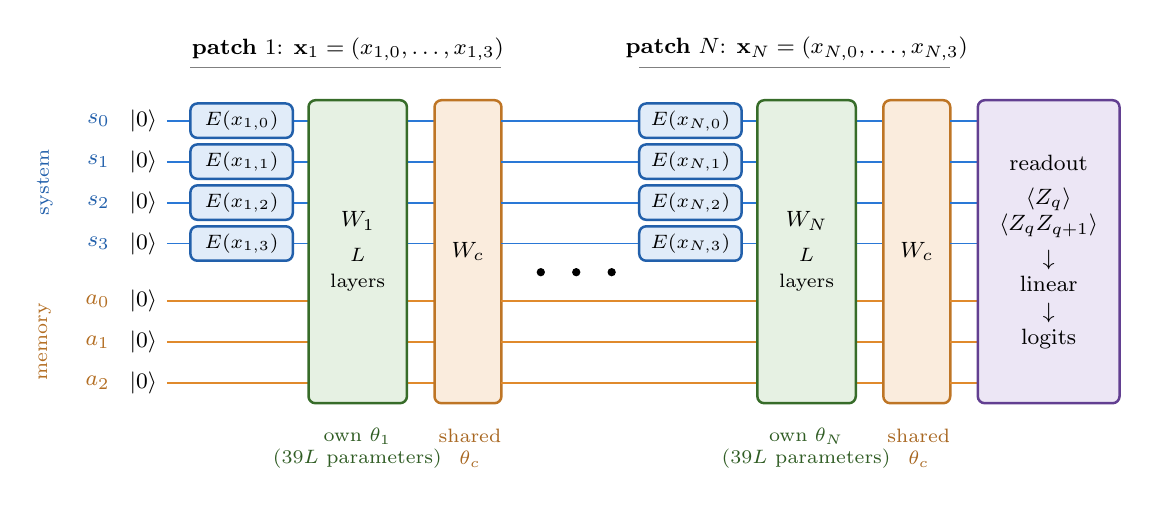
\begin{tikzpicture}[x=1cm,y=-0.52cm,font=\footnotesize,
  wire/.style={line width=0.7pt},
  blk/.style={draw,rounded corners=2.5pt,line width=0.9pt},
  ys/.style={draw=qblue!80!black,fill=qblue!14},
  yw/.style={draw=qgreen!70!black,fill=qgreen!14},
  yc/.style={draw=qorange!85!black,fill=qorange!16},
  yr/.style={draw=qpurple!80!black,fill=qpurple!14}]
  % wires: y positions of s0..s3 and a0..a2
  \def\ysys{0,1,2,3}
  \def\yanc{4.4,5.4,6.4}
  \def\H{7.5} % bottom of boxes
  \newcommand{\patch}[2]{% #1 = x offset, #2 = patch label
    \begin{scope}[xshift=#1 cm]
      \foreach \y in \ysys {\draw[wire,qblue] (-0.45,\y) -- (3.95,\y);}
      \foreach \y in \yanc {\draw[wire,qorange] (-0.45,\y) -- (3.95,\y);}
      \foreach \y in \ysys {\draw[blk,ys] (-0.15,\y-0.42) rectangle (1.15,\y+0.42) node[midway,font=\scriptsize] {$E(x_{#2,\y})$};}
      \draw[blk,yw] (1.35,-0.5) rectangle (2.6,6.9) node[midway,align=center] {$W_{#2}$\\[3pt]\scriptsize $L$\\\scriptsize layers};
      \draw[blk,yc] (2.95,-0.5) rectangle (3.8,6.9) node[midway,align=center] {$W_c$};
      \draw[line width=0.6pt,gray] (-0.15,-1.3) -- (3.8,-1.3);
      \node[above=-1pt] at (1.85,-1.3) {\textbf{patch} $#2$: $\mathbf{x}_{#2}=(x_{#2,0},\dots,x_{#2,3})$};
      \node[qgreen!60!black,align=center,font=\scriptsize] at (1.97,8.0) {own $\theta_{#2}$\\($39L$ parameters)};
      \node[qorange!75!black,align=center,font=\scriptsize] at (3.4,8.0) {shared\\$\theta_c$};
    \end{scope}}
  % labels and initial states
  \foreach \y/\l in {0/s_0,1/s_1,2/s_2,3/s_3} {\node[qblue!80!black,anchor=east] at (-1.05,\y) {$\l$};\node[anchor=east] at (-0.45,\y) {$|0\rangle$};}
  \foreach \y/\l in {4.4/a_0,5.4/a_1,6.4/a_2} {\node[qorange!80!black,anchor=east] at (-1.05,\y) {$\l$};\node[anchor=east] at (-0.45,\y) {$|0\rangle$};}
  \node[qblue!80!black,rotate=90,font=\scriptsize] at (-2.0,1.5) {system};
  \node[qorange!80!black,rotate=90,font=\scriptsize] at (-2.0,5.4) {memory};
  \patch{0}{1}
  % dots between patch 1 and patch N
  \foreach \y in \ysys {\draw[wire,qblue] (3.8,\y) -- (5.7,\y);}
  \foreach \y in \yanc {\draw[wire,qorange] (3.8,\y) -- (5.7,\y);}
  \foreach \x in {4.3,4.75,5.2} {\fill (\x,3.7) circle (1.5pt);}
  \patch{5.7}{N}
  % readout
  \foreach \y in \ysys {\draw[wire,qblue] (9.5,\y) -- (9.85,\y);}
  \foreach \y in \yanc {\draw[wire,qorange] (9.5,\y) -- (9.85,\y);}
  \draw[blk,yr] (9.85,-0.5) rectangle (11.65,6.9) node[midway,align=center] {readout\\[3pt]$\langle Z_q\rangle$\\$\langle Z_qZ_{q+1}\rangle$\\[3pt]$\downarrow$\\linear\\$\downarrow$\\logits};
\end{tikzpicture}
}
    \caption{Coherent memory. The same seven qubits are used for every patch. Each pixel $x_{i,k}$ of the $2\times2$ patch $\mathbf{x}_i$ is encoded on its own system qubit $s_k$ (blue) by the single-qubit map $E$ of Eq.~\eqref{eq:encoding}; $W_i$ (green, $L$ layers) has its own trainable parameters; $W_c$ (orange) is shared by all patches and couples the three ancilla qubits that carry the memory to the system; the readout (purple) measures expectation values and applies a linear layer.}
    \label{fig:circuit-coherent}
  \end{subfigure}

  \bigskip
  \begin{subfigure}{\textwidth}
    \centering
    \resizebox{\textwidth}{!}{% Serialized circuit with measured memory (Fig.~\ref{fig:measured}); colours defined in main.tex
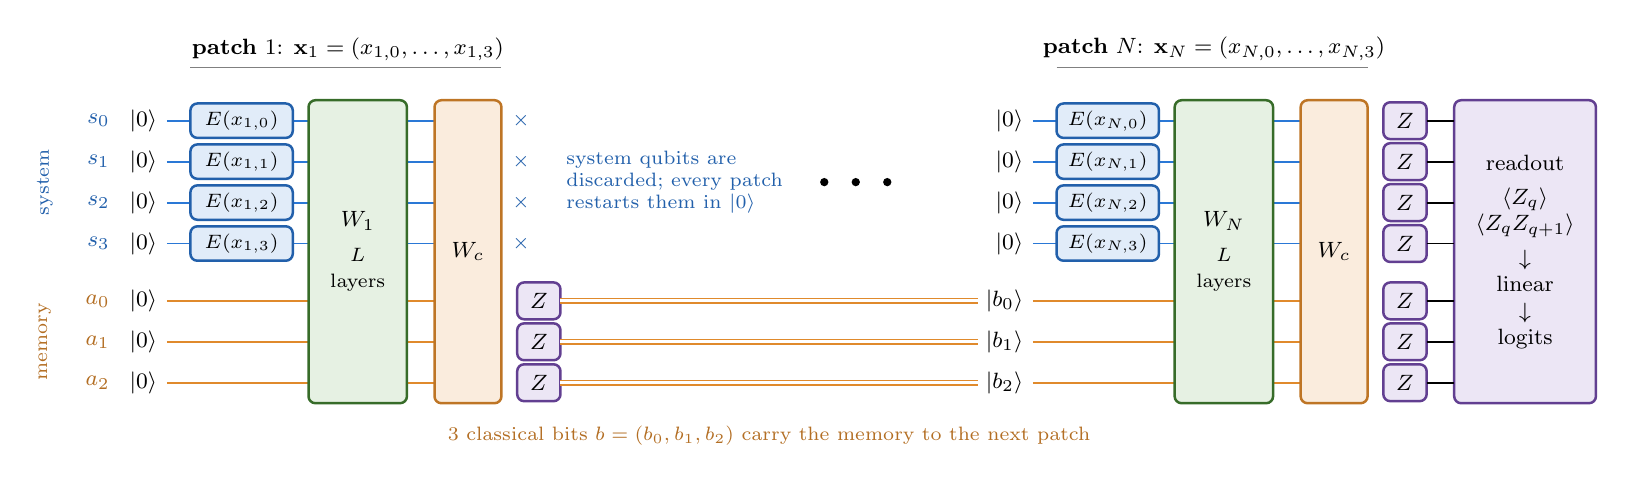
\begin{tikzpicture}[x=1cm,y=-0.52cm,font=\footnotesize,
  wire/.style={line width=0.7pt},
  cwire/.style={double=white,double distance=1.1pt,line width=0.6pt,draw=qorange},
  blk/.style={draw,rounded corners=2.5pt,line width=0.9pt},
  ys/.style={draw=qblue!80!black,fill=qblue!14},
  yw/.style={draw=qgreen!70!black,fill=qgreen!14},
  yc/.style={draw=qorange!85!black,fill=qorange!16},
  yr/.style={draw=qpurple!80!black,fill=qpurple!14}]
  \def\ysys{0,1,2,3}
  \def\yanc{4.4,5.4,6.4}
  % one patch: #1 x offset, #2 label, #3 ancilla input state, #4 = 1 if the system qubits are discarded afterwards (otherwise everything is measured)
  \newcommand{\patch}[4]{%
    \begin{scope}[xshift=#1 cm]
      \foreach \y in \ysys {\draw[wire,qblue] (-0.45,\y) -- (3.8,\y); \node[anchor=east] at (-0.45,\y) {$|0\rangle$};}
      \foreach \y/\i in {4.4/0,5.4/1,6.4/2} {\draw[wire,qorange] (-0.45,\y) -- (3.8,\y); \ifnum#4=1 \node[anchor=east] at (-0.45,\y) {$|0\rangle$};\else\node[anchor=east] at (-0.45,\y) {$|b_\i\rangle$};\fi}
      \foreach \y in \ysys {\draw[blk,ys] (-0.15,\y-0.42) rectangle (1.15,\y+0.42) node[midway,font=\scriptsize] {$E(x_{#2,\y})$};}
      \draw[blk,yw] (1.35,-0.5) rectangle (2.6,6.9) node[midway,align=center] {$W_{#2}$\\[3pt]\scriptsize $L$\\\scriptsize layers};
      \draw[blk,yc] (2.95,-0.5) rectangle (3.8,6.9) node[midway,align=center] {$W_c$};
      \draw[line width=0.6pt,gray] (-0.15,-1.3) -- (3.8,-1.3);
      \node[above=-1pt] at (1.85,-1.3) {\textbf{patch} $#2$: $\mathbf{x}_{#2}=(x_{#2,0},\dots,x_{#2,3})$};
      \ifnum#4=1
        \foreach \y in \yanc {\draw[blk,yr] (4.0,\y-0.45) rectangle (4.55,\y+0.45) node[midway] {$Z$};}
        \foreach \y in \ysys {\node[qblue!80!black,font=\scriptsize] at (4.05,\y) {$\times$};}
      \else
        \foreach \y in {0,1,2,3,4.4,5.4,6.4} {\draw[blk,yr] (4.0,\y-0.45) rectangle (4.55,\y+0.45) node[midway] {$Z$};}
      \fi
    \end{scope}}
  \node[qblue!80!black,rotate=90,font=\scriptsize] at (-2.0,1.5) {system};
  \node[qorange!80!black,rotate=90,font=\scriptsize] at (-2.0,5.4) {memory};
  \foreach \y/\l in {0/s_0,1/s_1,2/s_2,3/s_3} {\node[qblue!80!black,anchor=east] at (-1.05,\y) {$\l$};}
  \foreach \y/\l in {4.4/a_0,5.4/a_1,6.4/a_2} {\node[qorange!80!black,anchor=east] at (-1.05,\y) {$\l$};}
  \patch{0}{1}{}{1}
  % classical bits between patches (the system qubits are discarded and start again in |0>)
  \foreach \y in \yanc {\draw[cwire] (4.55,\y) -- (9.85,\y);}
  \node[qorange!80!black,font=\scriptsize,align=center] at (7.2,7.7) {3 classical bits $b=(b_0,b_1,b_2)$ carry the memory to the next patch};
  \node[qblue!80!black,font=\scriptsize,align=left,anchor=west] at (4.5,1.5) {system qubits are\\discarded; every patch\\restarts them in $|0\rangle$};
  \foreach \x in {7.9,8.3,8.7} {\fill (\x,1.5) circle (1.5pt);}
  \patch{11}{N}{}{0}
  \draw[blk,yr] (15.9,-0.5) rectangle (17.7,6.9) node[midway,align=center] {readout\\[3pt]$\langle Z_q\rangle$\\$\langle Z_qZ_{q+1}\rangle$\\[3pt]$\downarrow$\\linear\\$\downarrow$\\logits};
  \foreach \y in {0,1,2,3,4.4,5.4,6.4} {\draw[wire] (15.55,\y) -- (15.9,\y);}
\end{tikzpicture}
}
    \caption{Measured memory. The ancillas are measured in the $Z$ basis after every patch and the next patch starts from the measured bits $b=(b_0,b_1,b_2)$ (double lines are classical); the system qubits are discarded and restart in $\lvert0\rangle$. All seven qubits are measured after the last patch.}
    \label{fig:circuit-measured}
  \end{subfigure}
  \caption{The serialized circuit with its two kinds of memory between patches. The number of parameters grows with the number of patches; the number of qubits and the depth per patch do not.}
  \label{fig:circuit}
\end{figure}

Serialization is what reconciles a qubit encoding with a small register. At each patch step the four features occupy four distinct system qubits, each loaded by three rotations whose angles are trainable functions of $x$, $\sqrt{1-x^2}$ and $x^3$. There is no global vector normalization, so the preprocessed feature values enter the angles directly. The system qubits are then reused for the following patches, so all 196 pixels of a $14\times14$ image are processed sequentially on the same seven-qubit register, whereas an amplitude encoding on that register holds at most $2^7=128$ normalized values.

Because nothing is shared between $W_i$ and $W_j$ for $i\neq j$, which is what distinguishes the circuit from a recurrent quantum cell that reuses one transformation at every step, the number of trainable parameters,
\begin{equation}
  P_{\mathrm{Q}} = \underbrace{N\,L\,(6n-3)}_{W_1,\dots,W_N}+\underbrace{51}_{W_c}+\underbrace{24}_{E}+\underbrace{15k}_{\text{readout}}
  \label{eq:params}
\end{equation}
for $N$ patches, $L$ layers per block, $n=7$ qubits and $k$ classes, grows linearly with the size of the input while the number of qubits and the depth per patch stay fixed. For ten MNIST classes this gives 1\,473 and 2\,721 parameters at $8\times8$ ($N=16$, $L=2$ and $4$) and 4\,047 and 7\,869 at $14\times14$ ($N=49$), the size of small classical networks. Because of the usual redundancy of Euler-angle rotation layers, about 82--92\% of these parameters are independent directions at a random point (Methods). A circuit that loads the whole input at once on $n$ qubits, in contrast, has only $L(6n-3)$ quantum parameters whatever the input size, unless it re-uploads the input with new parameters~\cite{perezsalinas2020reuploading}. Only a small part of the total sits in the classical readout: the linear layer holds $15k$ parameters, $150$ of $2\,721$ for ten classes at $8\times8$ with $L=4$. The growth is a growth in parameters only; the total coherent depth, the simulation cost and, for the measured variant, the number of circuit executions still grow with $N$. The entanglement is local (nearest-neighbour controlled rotations inside a seven-qubit block and memory--system couplings) and all angles start close to the identity, in the spirit of identity-block initialization~\cite{grant2019initialization}, so adding parameters means adding patches or layers of the same small block, not building a deeper random circuit on more qubits, which is the setting in which barren plateaus are expected~\cite{mcclean2018barren}.

We study two ways of carrying information from one patch to the next. In the \emph{coherent} variant all qubits keep their state through the whole input, which on hardware requires coherence over all patches. In the \emph{measured} variant every patch is a short fresh circuit: the system qubits start in $\lvert0\rangle$, the ancillas are measured in the $Z$ basis after the patch, and the next patch starts from the measured bits. Only three classical bits, one of $2^3=8$ states, connect consecutive patches, and the depth that must stay coherent is that of one patch, which matches hardware with mid-circuit measurement and reset. Seen from the readout, the measured variant is a stochastic finite-state machine, an input-driven hidden Markov model over eight states whose transition probabilities are computed by the circuit of each patch; the coherent variant carries a seven-qubit quantum state instead. Both variants have the same encoding, blocks and parameter count, so comparing them isolates the role of the memory.

Encoding, readout and training are the same in every experiment. What varies is the number of parameters (through $L$ and $N$), the register size (through amplitude-encoding baselines on four and seven qubits, which also change how much of the input can be loaded and how many readout features there are) and the memory. Every neural model, quantum or classical, is trained for 100 epochs with the same optimizer, and we report the last epoch as the mean and standard deviation over three seeds (Methods).

\subsection{Gradients along the sequence of patches}
\label{sec:res-gradients}

Because every patch adds its own block, a natural concern is that the gradient with respect to the early blocks decays along the sequence, the serial counterpart of a barren plateau, so that the added parameters cannot be trained. We examined this on MNIST, downsampled to $8\times8$ and $14\times14$, with four tasks (3 vs.\ 5, 4 vs.\ 9, the digits 0--3 and all ten digits), 1\,000 training images per class and the full test set (Methods). The serialized circuit was run with $L\in\{2,4\}$ and both memory variants, and, as a non-serialized reference, the whole image was loaded as a normalized amplitude vector on 4 or 7 qubits and followed by 2, 4 or 8 layers of the same block and readout. In all 96 MNIST runs we recorded the whole-model gradient norm before clipping at every epoch, and the gradient norm of each $W_i$ on the first batch of epochs 1 and 100 (Fig.~\ref{fig:gradients}).

\begin{figure}[t]
  \centering
  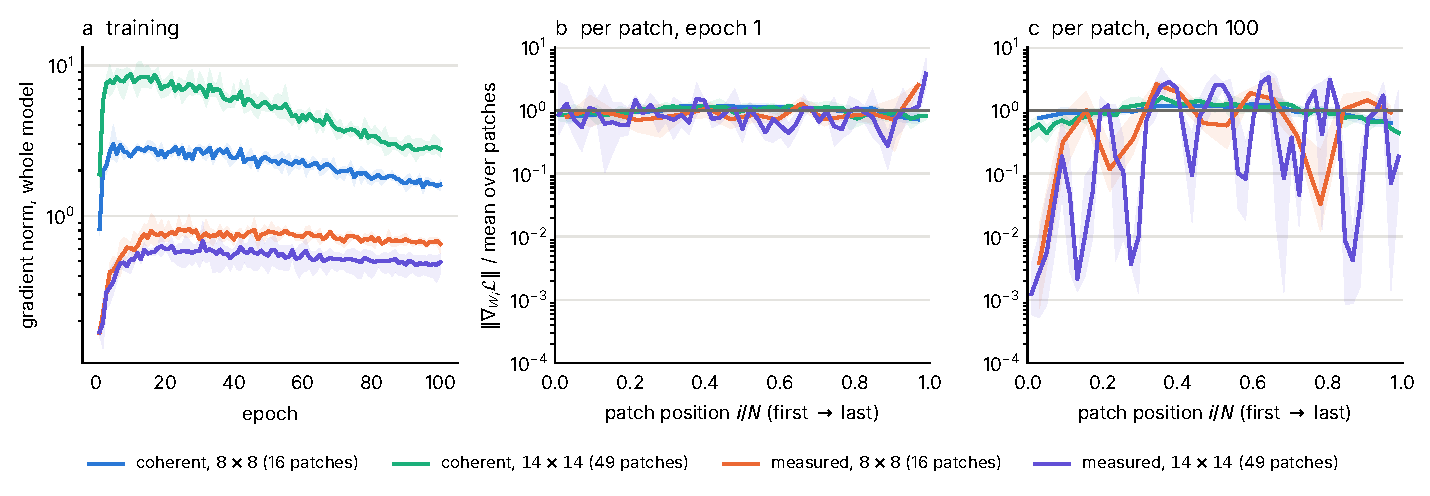
\includegraphics[width=\textwidth]{figures/fig_gradients.pdf}
  \caption{Trainability diagnostics, MNIST with ten classes and $L=4$ (lines: geometric mean over three seeds; bands: minimum to maximum; blue and green: coherent memory with 16 and 49 patches, orange and violet: measured memory with 16 and 49 patches). \textbf{a} Whole-model gradient norm before clipping (threshold 5), averaged over the batches of each epoch. \textbf{b, c} Gradient norm of each position-specific block $W_i$ on the first batch of epoch 1 and of epoch 100, divided by its mean over the patches, against the relative position $i/N$ of the patch in the sequence (16 patches at $8\times8$, 49 at $14\times14$). These values are read after clipping, which rescales all patches of a batch alike and therefore leaves the plotted ratios unchanged.}
  \label{fig:gradients}
\end{figure}

With coherent memory the gradients are spread evenly over the sequence (Fig.~\ref{fig:gradients}b,c). In every coherent run the smallest and the largest $W_i$ gradient differ by at most a factor of ten, and the earliest patches, whose gradient passes through the most subsequent steps, receive within a factor of about three as much gradient as the last ones, for 16 and for 49 patches alike. Tripling the number of patches therefore does not produce a collapse. The whole-model gradient norm stays within about two orders of magnitude throughout training (Fig.~\ref{fig:gradients}a), and the training loss falls by at least a factor of six in every run.

The measured circuit starts the same way, with no patch starved of gradient at epoch 1. By epoch 100, however, about 40\% of its patch positions receive less than a hundredth of the largest gradient of their run. These are mostly the border patches, which are nearly empty in MNIST, together with patches at the start of the sequence (Fig.~\ref{fig:gradients}c). The whole-model gradient norm of the measured circuit stays moderate at the end of training, so this is an uneven use of the patches that develops during training and not a vanishing gradient at initialization. Whether it reflects saturated measurement outcomes or patches that the model learns to ignore is not resolved by these data.

These observations support the empirical trainability of the tested seven-qubit circuits with coherent memory, with up to 49 patches and 7\,869 parameters; with measured memory a large part of the patch positions receives almost no gradient by the end of training. They are diagnostics of a few training trajectories and not a barren-plateau analysis. The register is fixed at seven qubits, where the concentration of gradients expected for random circuits, of order $2^{-n}$, is mild; all angles start close to the identity; and panels b and c show ratios to the mean over the patches, so the absolute scale is given only by the whole-model norm in panel a. We therefore also measured gradient statistics over random initializations as the register grows.

The register of the serialized circuit grows through its memory. We drew the untrained circuit 200 times for $n=5$ to $11$ qubits (four system qubits and one to seven memory qubits) and for $N=4$ and $16$ patches, evaluated it on a fixed batch of random inputs, and computed the variance over the draws of the gradient with respect to one angle of the first block $W_1$ (Fig.~\ref{fig:gradvar}; Methods). Two costs were used: a local one, $\langle Z_{s_0}\rangle$ on one system qubit, and a global one, the product of $Z$ over all $n$ qubits. With all block angles drawn uniformly from $[-\pi,\pi)$, the setting of the barren-plateau result for random circuits~\cite{mcclean2018barren}, the variance halves with every added qubit, for both costs and both sequence lengths. Serialization therefore does not protect the circuit from barren plateaus. With the near-identity initialization used in every training run the picture changes: the variance of the local cost stays at about $10^{-2}$ over the whole range, while that of the global cost still decreases with $n$, slowly for four patches and faster for sixteen. The gradient with respect to the last block $W_N$ behaves in the same way. The number of patches matters much less than the number of qubits. Going from $N=4$ to $16$ patches quadruples the block parameters but lowers the local-cost variance of the first block by less than a factor of two at the near-identity start and leaves that of the last block unchanged, and from random angles the variance is the same for both lengths at every $n$. In this circuit the parameter count can therefore grow through patches, each a shallow block, without a further loss of gradient, while the size of the register sets the exponential decay. This agrees with the known mitigation of barren plateaus by local costs and by initialization close to the identity~\cite{cerezo2021costbp,grant2019initialization}: the readout of the circuit consists of one- and two-qubit terms, and the trainability seen in the training runs rests on these two choices and not on the serial structure itself. Eleven qubits are still small, so the data show the trend over this range and not its asymptotic form.

\begin{figure}[t]
  \centering
  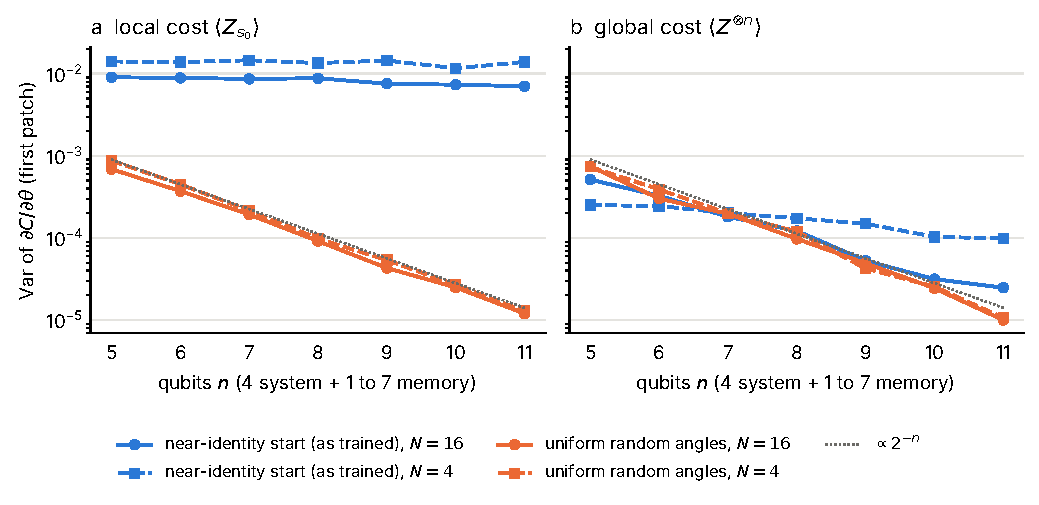
\includegraphics[width=\textwidth]{figures/fig_gradvar.pdf}
  \caption{Variance of the gradient over 200 random initializations of the untrained serialized circuit, against the number of qubits $n$ (four system qubits and $n-4$ memory qubits; $L=4$, coherent memory, the same 16 random inputs for every draw). The derivative is taken with respect to the $R_Y$ angle of the first $\mathrm{Rot}$ on $s_0$ in the first block $W_1$. Blue: all angles from $\mathcal{N}(0,0.08^2)$ as in the training runs; orange: block angles uniform in $[-\pi,\pi)$. Solid: $N=16$ patches; dashed: $N=4$. Dotted: a line proportional to $2^{-n}$. \textbf{a} Local cost $\langle Z_{s_0}\rangle$. \textbf{b} Global cost $\langle Z^{\otimes n}\rangle$.}
  \label{fig:gradvar}
\end{figure}

\subsection{Effects of parameter count and register size on MNIST}
\label{sec:res-capacity}

Given these gradients, we ask what the added parameters buy. On MNIST, accuracy grows with the number of trainable parameters of the serialized circuit, for both memory variants (Fig.~\ref{fig:capacity}). Doubling the layers per patch at a fixed image size helps the coherent circuit by about a point on the binary and 10-class tasks and not at all on 4 classes; it helps the measured circuit in every case and by much more, up to about six points. Adding patches, by going from $8\times8$ to $14\times14$ images, also adds parameters at the same seven qubits and raises the accuracy, on 10 classes with $L=4$ by about two points with coherent and five with measured memory; since it also raises the resolution of the input, it reflects capacity and information together. On the binary tasks at $14\times14$ the coherent circuit fits the training set almost perfectly, so its remaining error there is a generalization gap and not a lack of capacity. All accuracies are in Supplementary Tables~\ref{tab:mnist-results} and~\ref{tab:mnist-amp}.

\begin{figure}[t]
  \centering
  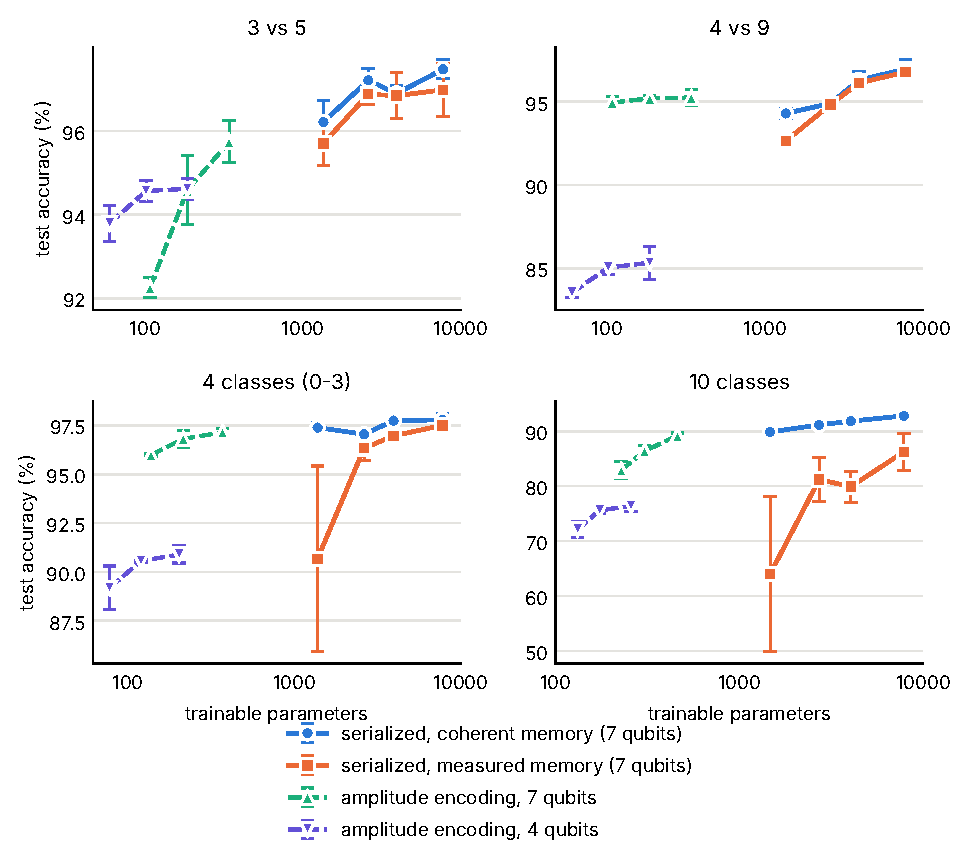
\includegraphics[width=0.78\textwidth]{figures/fig_capacity.pdf}
  \caption{Test accuracy against the number of trainable parameters on MNIST (mean $\pm$ standard deviation over three seeds). Solid: serialized circuit on 7 qubits with coherent (blue) and measured (orange) memory; the four points of each are $8\times8$ and $14\times14$ images with $L=2$ and $L=4$, from fewest to most parameters. Dashed: amplitude-encoding circuits on 7 and on 4 qubits for $14\times14$ inputs with $L=2,4,8$ layers of the same block. Accuracy rises with the parameter count and with the number of qubits.}
  \label{fig:capacity}
\end{figure}

The register size enters through the amplitude-encoding circuits, which vary it with the same block, readout form and training. A larger register also lets more of the input be loaded and gives more readout features, so these results do not isolate the number of qubits alone. Seven qubits beat four at every depth on 4 vs.\ 9, 4 classes and 10 classes, by 6 to 13 points, while 3 vs.\ 5 is already close to saturation on four qubits. The gain is not only a matter of parameters: at approximately matched parameter counts the 7-qubit circuit is still ahead on the three harder tasks by 6 to 10 points. With amplitude encoding the register also bounds how much of the image can be loaded ($16$ against $121$ values), which is the restriction that processing the features patch by patch removes.

The serialized circuit processes all pixels on the same seven qubits, and its parameter count is not tied to the register (up to 7\,869 parameters, against at most 462 for the amplitude circuits). At $14\times14$ with $L=4$ it is ahead of the 7-qubit amplitude circuit on all four tasks, most on 10 classes. In the tested configurations a larger register and more parameters therefore both go with higher accuracy, and the serialized circuit has the second without needing the first to grow with the input.

The memory behaves differently on easy and hard tasks. On the binary tasks and on 4 classes measured memory is mostly within a point of coherent memory; the exceptions are the two smallest circuits ($8\times8$, $L=2$) on 4 vs.\ 9 and 4 classes. On 10 classes it is clearly behind, by about 7 to 12 points in the three larger circuits. In the smallest of these cells one of the three seeds stalled early in training and is included in the mean; it stalls also with two other sets of initial angles but not with another draw of training images, so it depends on the images or their order and not on the initialization. Training accuracy is about equal to test accuracy in these runs, so within the 100-epoch budget the measured circuit underfits rather than overfits. Doubling $L$ raises its training accuracy on 10 classes at $8\times8$ by 18 points, so slower optimization may contribute as well; longer training was not tested. This is consistent with the restrictive information bottleneck of a three-bit measured memory, but it does not imply a general relation between the number of memory states and the number of classes that can be learned, since the last patch, the system register and the readout also carry information.

\subsection{Comparison with classical models of the same size}
\label{sec:res-classical}

To put these numbers in context we compare the circuit with a one-hidden-layer MLP and a small CNN that have the same number of parameters (Fig.~\ref{fig:classical}).

\begin{figure}[t]
  \centering
  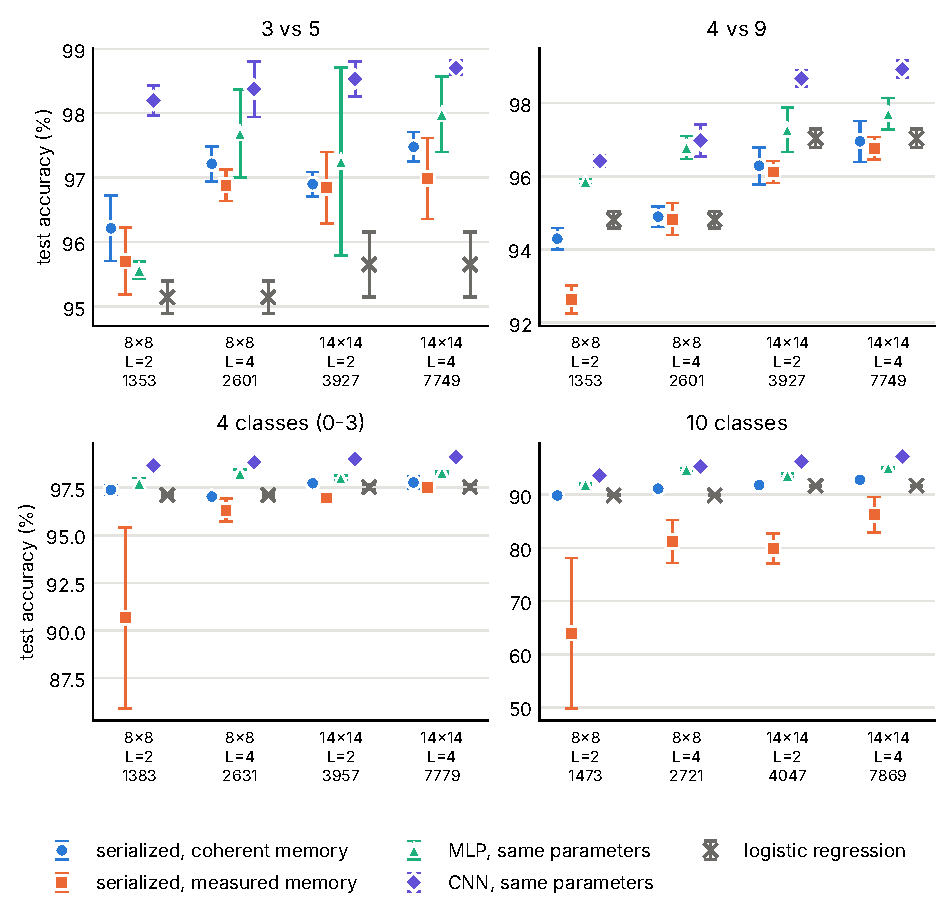
\includegraphics[width=0.78\textwidth]{figures/fig_classical.pdf}
  \caption{MNIST: serialized circuit (coherent and measured memory) against classical models with the same number of parameters (MLP and CNN, sized to the circuit; the parameter count of the circuit is printed under each group) and against logistic regression (which has its own, smaller size). Test accuracy, mean $\pm$ standard deviation over three seeds.}
  \label{fig:classical}
\end{figure}

With coherent memory the circuit is level with logistic regression or slightly above it on every task except 4 vs.\ 9, where it is slightly below. Against the parameter-matched MLP it ranges from slightly ahead to about two points behind on the 2- and 4-class tasks, and it is two to four points behind on 10 classes. The CNN, whose convolutions build in the translation structure of images, is better still. Measured memory is within about a point of the MLP on the binary and 4-class tasks at $14\times14$ but well behind it on 10 classes. Once the parameter count is matched, the serialized circuit thus comes close to the classical MLP on the easier tasks with seven qubits. All numbers are in Supplementary Table~\ref{tab:mnist-results}.

\subsection{Twelve further datasets}
\label{sec:res-datasets}

To see whether these findings carry over, we fixed the architecture and training recipe (coherent memory, $L=4$, the same encoding, readout and training) and applied it, retraining all parameters, to twelve further datasets: eight tabular sets with 16 to 57 features (4 to 15 patches) and four image sets at $14\times14$ (49 patches) with 2 to 26 classes (Supplementary Table~\ref{tab:datasets}; Methods). The only dataset-dependent setting is the initial encoding scale. Measured memory was run on the eight tabular sets only, since on the 49-patch image sets it would take days per run. Fig.~\ref{fig:bench} shows the test accuracy of each model relative to the MLP with approximately the same number of parameters (within $2.5\%$).

\begin{figure}[t]
  \centering
  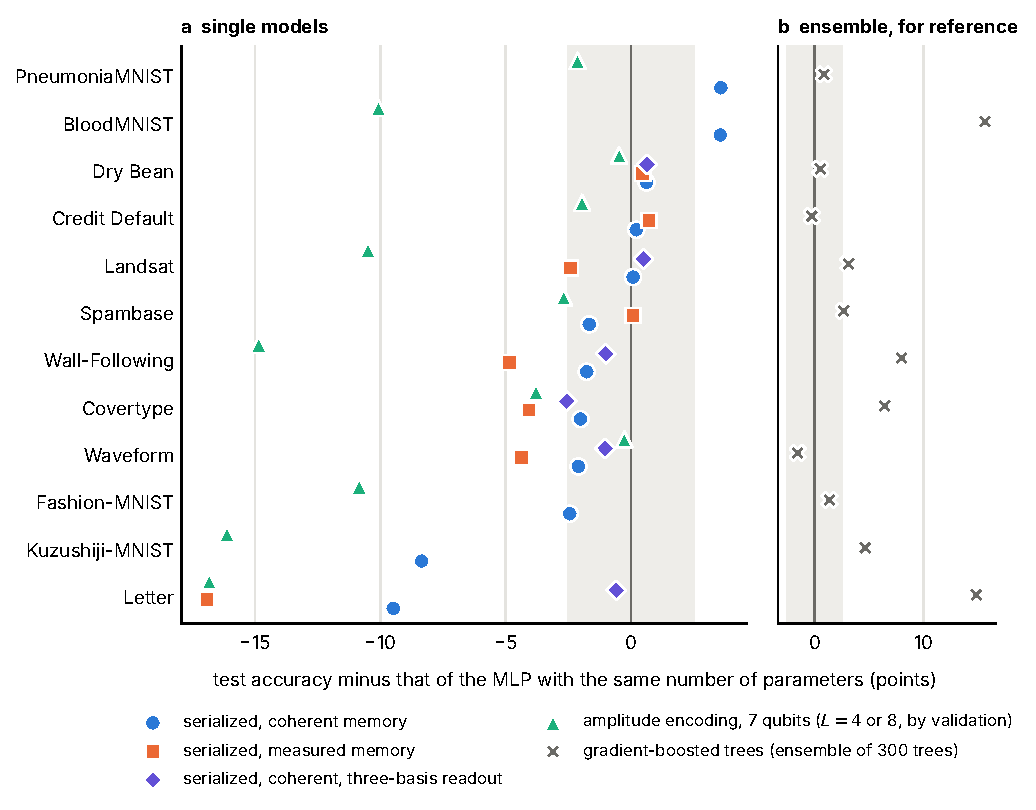
\includegraphics[width=0.8\textwidth]{figures/fig_bench.pdf}
  \caption{Test accuracy on the twelve further datasets, relative to the one-hidden-layer MLP with the same number of parameters as the circuit (zero line); the shaded band is $\pm2.5$ points. Datasets are ordered by the difference between the coherent circuit and the MLP; all accuracies are in Supplementary Table~\ref{tab:bench}. \textbf{a} Single models: the serialized circuit (blue circles: coherent memory; orange squares: measured memory; violet diamonds: coherent memory with the three-basis readout of Table~\ref{tab:readout}, run on the six tabular sets with three or more classes, whose larger linear head gives it 8--65\% more parameters than the MLP of the zero line) and amplitude encoding on the same seven qubits, with the depth of higher validation accuracy (green triangles). \textbf{b} Gradient-boosted trees, an ensemble of 300 trees, shown on its own axis as a reference; boosting can be applied to the circuit as well (Discussion).}
  \label{fig:bench}
\end{figure}

Against the MLP of the same size the circuit is close on most datasets. On eight of the twelve it lies inside the band of $\pm2.5$ points, slightly behind on Waveform, Wall-Following, Covertype, Spambase and Fashion-MNIST and level or slightly ahead on Credit Default, Landsat and Dry Bean. It is ahead on BloodMNIST and PneumoniaMNIST and clearly behind, by about nine points, on Letter (26 classes from 16 features) and Kuzushiji-MNIST. On the image sets a CNN of the same size, whose convolutions build in the structure of images, stays ahead except on PneumoniaMNIST. Balanced accuracy, which weights the classes equally (Supplementary Table~\ref{tab:bench-bal}), changes the picture only on Covertype, where the largest class holds almost half of the examples and the circuit falls well outside the band.

The band is a descriptive threshold and not an equivalence test, so we also asked which differences exceed the sampling error of the fixed test sets. For a single model this error is larger than the spread over seeds (a binomial standard error of $0.4$ to $1.3$ points), and the advantage on PneumoniaMNIST, with only 624 test images, is within it. Because both models are scored on the same examples, a paired test is sharper: an exact McNemar test on reruns with stored predictions (Methods) finds no significant difference on Credit Default, Landsat and Dry Bean, while the small deficits on Waveform, Wall-Following, Covertype and Spambase are significant ($p\le0.05$). Inside the band the circuit therefore matches the MLP on three tabular sets and is slightly but measurably behind it on four. On Credit Default, where 78\% of the examples are in one class, accuracy says little in any case.

Gradient-boosted trees are shown on their own axis (Fig.~\ref{fig:bench}b) because they are an ensemble of 300 trees and not a single model of the size of the circuit; the circuit itself could serve as the weak learner of a boosted ensemble, and quantum ensemble and boosting methods have been proposed~\cite{schuld2018ensembles,arunachalam2020boosting}. Untuned, the trees are the strongest model on 8 of the 12 sets, in line with reports that tree-based models remain strong on medium-sized tabular data~\cite{grinsztajn2022trees}, and far ahead where features need sharp thresholds, as on Wall-Following and Letter, whereas on Credit Default, Dry Bean and PneumoniaMNIST the single circuit is level with them or ahead.

The comparison with amplitude encoding on the same seven qubits (with the depth, $L=4$ or $8$, of higher validation accuracy) is the clearest in favour of the circuit. The serialized circuit is better on 11 of the 12 datasets, by more than five points on seven of them and by up to $13.6$ points on BloodMNIST, and behind only on Waveform. Deeper amplitude circuits close none of the large gaps, because their parameter count does not grow with the input while that of the serialized circuit does. The two models also differ in parameter count and in how much of the input they represent, so this compares architectures and does not isolate serialization.

The two memory variants separate on the tabular sets in the same way as on MNIST. Coherent memory is better on five of the six sets with three or more classes, most clearly on Letter, the two are level on Dry Bean, and measured memory is slightly better on the two binary sets, Spambase and Credit Default. The quantum link between patches thus helps most where many classes must be separated, while for the binary tasks the three-bit classical link was enough. Measured runs also vary more across seeds (Supplementary Table~\ref{tab:bench}).

\subsection{Reading out more than the computational basis}
\label{sec:res-readout}

The largest remaining gaps are on Letter and Kuzushiji-MNIST, but they look different. On Kuzushiji-MNIST the training accuracy of the circuit is $17.0$ points above its test accuracy, so the gap there is mainly one of generalization. On Letter the two differ by only $0.8$ points: the circuit underfits, with 26 classes to be separated by a linear layer that sees only 14 features. We therefore kept the circuit fixed and gave the linear layer the same quantities in all three Pauli bases, $\langle Z_q\rangle$, $\langle Z_qZ_{q+1}\rangle$, $\langle X_q\rangle$, $\langle X_qX_{q+1}\rangle$, $\langle Y_q\rangle$ and $\langle Y_qY_{q+1}\rangle$ (42 features), on the tabular sets with more than four classes, two small-class checks and MNIST (Table~\ref{tab:readout}).

On Letter the test accuracy rises by about nine points (diamonds in Fig.~\ref{fig:bench}). The larger readout also enlarges the linear layer, so we ran a control with the original readout and a deeper circuit, $L=9$, with about the same number of parameters; it gains less than a point. The training accuracy moves in the same way, so the gain is in what the model can fit and not only in how it generalizes. On every other dataset the change is within about a point, comparable to the spread over seeds. MLPs re-sized to the 42-feature circuit gain on Letter as well, so the ranking against classical models does not change. On hardware the $X$ and $Y$ terms require two further measurement settings, that is three times the shots, while the circuit itself is unchanged.

\begin{table}[t]
  \centering
  \caption{Readout in three Pauli bases. Test accuracy (\%), mean $\pm$ standard deviation over three seeds, parameters in brackets; circuit with coherent memory and $L=4$. The MLP is re-sized to the parameter count of the 42-feature circuit. The best mean of each row is in bold. Control: $Z$, $ZZ$ readout with $L=9$ (1\,869 parameters): $71.8\pm2.1$ on Letter (Supplementary Table~\ref{tab:letter}).}
  \label{tab:readout}
  \footnotesize
  % generated by scripts/paper_figures.py -- do not edit
\begin{tabular}{@{}lrlllr@{}}
\toprule
dataset & $k$ & $Z$, $ZZ$ (14 features) & $+X$, $XX$, $Y$, $YY$ (42) & gain & MLP, size of 42-feature circuit \\
\midrule
MNIST $8\times8$ & 10 & $91.1\pm0.3$ (2\,721) & $92.0\pm0.4$ (3\,001) & $+0.9$ & $\mathbf{94.5}\pm0.4$ \\
Letter & 26 & $71.0\pm1.6$ (1\,089) & $79.9\pm0.2$ (1\,817) & $+8.9$ & $\mathbf{84.7}\pm1.2$ \\
Covertype & 7 & $73.8\pm0.2$ (2\,364) & $73.2\pm0.5$ (2\,560) & $-0.6$ & $\mathbf{75.3}\pm0.2$ \\
Landsat & 6 & $89.3\pm1.2$ (1\,569) & $\mathbf{89.7}\pm0.2$ (1\,737) & $+0.4$ & $89.6\pm0.2$ \\
Dry Bean & 7 & $\mathbf{92.9}\pm0.2$ (804) & $\mathbf{92.9}\pm0.2$ (1\,000) & $+0.0$ & $92.6\pm0.2$ \\
Wall-Following & 4 & $90.1\pm0.7$ (1\,071) & $\mathbf{90.9}\pm1.5$ (1\,183) & $+0.8$ & -- \\
Waveform & 3 & $85.0\pm0.2$ (1\,056) & $\mathbf{86.0}\pm0.6$ (1\,140) & $+1.1$ & -- \\
\bottomrule
\end{tabular}

\end{table}

\subsection{Controls that remove one part of the circuit}
\label{sec:res-controls}

The comparisons so far do not show which parts of the circuit produce its accuracy. We therefore changed one part of the coherent $L=4$ circuit at a time, with the rest of the recipe fixed, on six tabular sets and on MNIST $8\times8$ with 3 vs.\ 5 and with ten classes (Table~\ref{tab:controls}; Methods). Changes are compared seed by seed with the main runs.

\begin{table}[t]
  \centering
  \caption{Controls of the coherent circuit with $L=4$. Test accuracy (\%), mean $\pm$ standard deviation over three seeds; $k$ classes, $N$ patches. Tied blocks: one block $W$ reused at every patch. Tied, same parameters: the tied block with $NL$ layers, which restores the parameter count, run on the sets with four to six patches. Product gates: every $\mathrm{CRot}$ replaced by a $\mathrm{Rot}$ on its target with the same angles, so that the state stays a product state and the parameter count is unchanged. Frozen random: block angles uniform in $[-\pi,\pi)$, encoding at its initial values, only the linear head trained. Feature order: change of the test accuracy, seed 42, for three random orders of the tabular features against the file order.}
  \label{tab:controls}
  \footnotesize
  \setlength{\tabcolsep}{4pt}
  \resizebox{\textwidth}{!}{% generated by scripts/paper_figures.py -- do not edit
\begin{tabular}{@{}lrrrrrrrr@{}}
\toprule
dataset & $k$ & $N$ & circuit & tied blocks & tied, same params & product gates & frozen random & feature order \\
\midrule
Waveform & 3 & 6 & $85.0${\scriptsize$\pm0.2$} & $84.8${\scriptsize$\pm0.8$} & $85.7${\scriptsize$\pm0.9$} & $81.6${\scriptsize$\pm0.5$} & $50.7${\scriptsize$\pm2.6$} & $-0.8$ to $+0.7$ \\
Wall-Following & 4 & 6 & $90.1${\scriptsize$\pm0.7$} & $84.5${\scriptsize$\pm0.5$} & $85.3${\scriptsize$\pm0.5$} & $81.4${\scriptsize$\pm0.9$} & $52.6${\scriptsize$\pm1.0$} & $+0.5$ to $+1.6$ \\
Letter & 26 & 4 & $71.0${\scriptsize$\pm1.6$} & $61.8${\scriptsize$\pm0.8$} & $64.7${\scriptsize$\pm1.2$} & $48.2${\scriptsize$\pm0.5$} & $30.3${\scriptsize$\pm0.8$} & $+3.1$ to $+5.8$ \\
Dry Bean & 7 & 4 & $92.9${\scriptsize$\pm0.2$} & $92.5${\scriptsize$\pm0.1$} & $92.8${\scriptsize$\pm0.2$} & $92.0${\scriptsize$\pm0.5$} & $75.5${\scriptsize$\pm1.8$} & $+0.0$ to $+0.1$ \\
Landsat & 6 & 9 & $89.3${\scriptsize$\pm1.2$} & $86.2${\scriptsize$\pm0.9$} & -- & $84.0${\scriptsize$\pm1.9$} & $55.1${\scriptsize$\pm4.0$} & $+1.4$ to $+1.8$ \\
Spambase & 2 & 15 & $91.7${\scriptsize$\pm0.4$} & $88.3${\scriptsize$\pm0.9$} & -- & $91.1${\scriptsize$\pm1.1$} & $64.7${\scriptsize$\pm1.1$} & $+1.0$ to $+2.1$ \\
MNIST $8\times8$, 3 vs.\ 5 & 2 & 16 & $97.2${\scriptsize$\pm0.3$} & $94.2${\scriptsize$\pm0.7$} & -- & $95.3${\scriptsize$\pm0.2$} & $59.2${\scriptsize$\pm1.4$} & -- \\
MNIST $8\times8$, 10 classes & 10 & 16 & $91.1${\scriptsize$\pm0.3$} & $79.6${\scriptsize$\pm1.7$} & -- & $74.5${\scriptsize$\pm0.5$} & $22.8${\scriptsize$\pm1.7$} & -- \\
\bottomrule
\end{tabular}
}
\end{table}

\paragraph{Position-specific blocks.}
Reusing one block at every patch, as a recurrent quantum cell does, lowers the mean accuracy on all eight tasks. The loss is marginal on Waveform and Dry Bean, a few points on Landsat, Spambase, Wall-Following and MNIST 3 vs.\ 5, and large on the two tasks with many classes, Letter and MNIST with ten classes. The tied circuit also has $N$ times fewer block parameters, so on the four sets with four to six patches we also ran a tied block $N$ times deeper, with the parameter count of the original circuit. It recovers the loss on Waveform and Dry Bean and part of it on Letter, but not on Wall-Following. On the harder tasks, giving each position its own parameters is thus worth more than the same number of parameters in one deeper shared block.

\paragraph{Entangling gates.}
Replacing every controlled rotation by a single-qubit rotation with the same angles keeps the parameter count but removes all interaction between qubits: each system qubit then sees only the features in its own position of every patch, the memory qubits do not see the input at all, and the $ZZ$ features factorize. The accuracy falls on all eight tasks, by about a point on Spambase and Dry Bean, by a few points on MNIST 3 vs.\ 5, Waveform, Landsat and Wall-Following, and by about twenty points on MNIST with ten classes and on Letter. Bowles et al.\ found that removing entanglement often did no harm in their models~\cite{bowles2024better}. Here it does harm, most on the tasks with many classes; since the product control removes the link through the memory together with the entanglement, it shows that interactions between the qubits matter, not that entanglement as such is a resource.

\paragraph{Training the circuit.}
With the circuit frozen at random angles and only the linear head trained, the accuracy drops far more than in any other control, by 17 to 68 points, most on MNIST with ten classes, where it falls to about a quarter of that of the trained circuit. The random features of a seven-qubit circuit are therefore far from enough, and the accuracy comes from training the circuit. Random angles are the regime in which the gradients concentrate (Fig.~\ref{fig:gradvar}), and the readout features concentrate in the same way, so the control is a weak random-feature model; it does not show that no fixed quantum feature map could do better.

\paragraph{Feature order.}
The tabular features enter in the order of the data file. Three random orders (seed 42) leave Waveform and Dry Bean essentially unchanged but raise the accuracy on the other four sets, on every order, by up to about six points on Letter. The file order was therefore not favourable to the circuit, and on Letter part of its gap to the MLP depends on the order of the features, which the MLP does not see.

\paragraph{Classical models with the structure of the circuit.}
The MLP sees all features at once. We therefore also trained three classical models that read the input patch by patch with position-specific parameters, as the circuit does: a recurrent network with its own weights at every step and a matrix-product-state classifier with one tensor per feature, both sized as close as their hidden or bond dimension allows to the parameter count of the circuit (within $8\%$ and $21\%$; the matrix-product state has about $20\%$ fewer parameters on the image sets), and an input-driven hidden Markov model with eight states, the classical counterpart of the measured circuit, whose size is fixed by its states (Supplementary Table~\ref{tab:struct}; Methods). On the tabular sets the recurrent network and the matrix-product state are about as accurate as the MLP and ahead of the circuit on most sets. On the 49-patch image sets, however, the circuit is ahead of both, clearly on Kuzushiji-MNIST and slightly on BloodMNIST and Fashion-MNIST, and level on PneumoniaMNIST, whereas on MNIST $8\times8$ with 16 patches it is about a point behind the better of the two. The eight-state Markov model is the weakest model on every set. The measured circuit, which carries the same eight states between patches, is ahead of it on seven of the eight tabular sets and on both MNIST tasks, although the Markov model has $1.5$ to $2$ times as many parameters; how the transition probabilities are parameterized therefore matters, and the circuit computes useful ones.

%\input{discussion}
%%%%%%%%%%%%%%%%%%%%%%%%%%%%%%%%%%%%%%%%%%%%%%%%%%%%%%%%%%%%%%%%%%%%%%%%%%%5

% Discussion section. Included from main.tex with \input{discussion}.
\section{Discussion}
\label{sec:discussion}

The experiments show that serialization decouples the number of trainable parameters from the size of the register. On a fixed register of seven qubits, with a fixed encoding, readout and training recipe, accuracy generally rises with the number of trainable parameters, whether they are added as layers per patch or as patches (the latter also raises the resolution of the input, so it does not isolate capacity), and the added parameters remain trainable: with coherent memory the gradients of the position-specific blocks do not decay along sequences of up to 49 patches. The serial structure does not cause this by itself. From random angles the gradients of the circuit vanish exponentially with the register, as in other random circuits; from the near-identity start used here, and with a local cost, they did not shrink between five and eleven qubits. The register size appears to matter as well, although it was varied only in the amplitude-encoding baselines and at two sizes. Among amplitude-encoding circuits, seven qubits did better than four also at approximately equal parameter counts, although the register size there also changes how much of the input can be loaded. Serialization combines the two effects, since it lets the parameter count follow the input without enlarging the register. Against amplitude encoding on the same seven qubits the serialized circuit is better by up to 13.6 points and on 11 of 12 datasets, and on MNIST on all four tasks. Because the two models differ in parameter count and represented input as well as in encoding, this is a comparison of architectures.

With approximately matched parameter counts, the gap to a classical MLP is within 2.5 points on 8 of the 12 further datasets (7 of 12 in balanced accuracy), and the circuit is ahead on two. Part of the usual gap between quantum and classical classifiers may therefore be associated with the number of parameters and with how the features are mapped to qubits, which these experiments do not separate from each other, rather than with an intrinsic weakness of parameterized circuits. This does not amount to a quantum advantage, and none is claimed: the classical models used here are small, a same-size CNN stays ahead on the image sets, and an ensemble of gradient-boosted trees is stronger still on 8 of the 12 datasets.

These results can be read alongside the benchmark of Bowles, Ahmed and Schuld~\cite{bowles2024better}, which is often cited as evidence that quantum classifiers do not beat classical ones. Our results do not contradict it, since the circuit studied here does not beat a classical model of the same size either, but the two studies ask different questions. Their quantum models were tuned by extensive hyperparameter searches and compared with out-of-the-box classical models whose parameter counts were deliberately not matched, since the authors did not consider matching components such as the number of parameters meaningful in their context, ``much like one does not enforce the same number of parameters when comparing kernel methods with neural networks''~\cite{bowles2024better}. Here the recipe is fixed and the parameter count is the variable, which is what allows part of the gap to be associated with it. Two of their observations agree with ours. In their benchmark the models based on amplitude encoding struggled even when given copies of the input, and amplitude encoding is also the weaker architecture here; for one of these models they point out that its number of parameters grows only logarithmically with the input, which fits our reading that the parameter count matters. They also note that results on small datasets cannot be extrapolated to larger ones and call for studies of scaling; the size of their circuits was limited by simulation cost, and serialization offers one way to grow the input and the parameter count while the register stays at seven qubits. The two studies also use different data, so the comparison is indirect; running the serialized circuit on their datasets and under their protocol would make it direct. Their finding that removing entanglement often does no harm does not hold for the serialized circuit, whose accuracy falls on every task we tested when the entangling gates are replaced by product gates, by up to 23 points; in this circuit, however, the same gates also carry the information between patches, so the two results concern different roles of the entangling gates.

These observations point to a more general constraint. Serialization frees the number of parameters from the register, but not the amount of information that leaves the circuit. With local Pauli readout in one basis, an $n$-qubit register gives $2n$ features, 14 here, however many parameters the circuit has, and the classical head can work only with these. When the number of classes approaches or exceeds this dimension, the readout rather than the circuit is expected to limit the model, and adding parameters inside the circuit cannot widen it. Letter, the only task here with more classes than readout features (26 against 14), fits this picture. The circuit underfits, with training and test accuracy within a point of each other; a deeper circuit with as many parameters as the larger readout gains about a point, whereas reading out the same state in three Pauli bases (42 features) gains about nine, in training as in test accuracy, and a classical MLP head on the 14 features lifts the circuit to within about two points of an MLP of the same size (Supplementary Table~\ref{tab:letter}). The MLP head shows that the 14 features carry more information about the classes than a linear map extracts, so on Letter the limit lies in the readout as a whole, the number of measured features together with the linear head, and not in the 14 numbers alone; with a non-linear head, however, much of the model is classical. On the six tasks with ten or fewer classes the three-basis readout changed the accuracy by about a point at most, comparable to the spread over seeds. The width of the readout is set by the register and by the number of measurement settings, so it is a further way, besides how much of the input can be loaded, in which the register size enters; in the amplitude-encoding comparison the four-qubit circuits also had fewer readout features (8 against 14), and these experiments do not separate the two. Kuzushiji-MNIST does not fit the same picture: with ten classes it has fewer classes than readout features, and its training accuracy is $17.0$ points above its test accuracy, so its gap is mainly one of generalization, which a wider readout would not be expected to close. More measurement bases cost three times the shots on hardware but no change to the circuit, so they are worth testing whenever a circuit underfits a task with many classes.

The memory between patches shows a similar dependence on the task. Measured memory occasionally improves generalization, most notably on Spambase. This may reflect its role as an information bottleneck: compressing previous patches into an eight-state classical channel can suppress unnecessary long-range correlations and simplify learning when coherent history is not required. However, the effect is dataset-dependent, and the present experiments do not yet distinguish this explanation from feature-order, optimization, and readout effects. On Spambase the measured circuit has a smaller gap between training and test accuracy than the coherent one ($1.8$ against $4.4$ points), which is consistent with this reading. Where many classes must be separated, the same bottleneck limits the model: on MNIST with ten classes and on Letter, measured memory underfits, with training accuracy close to test accuracy. The link between patches is thus a second channel whose width, three bits, is set by the register and not by the number of parameters, although more parameters per patch partly compensate: on MNIST with ten classes at $8\times8$, doubling $L$ raises the training accuracy of the measured circuit by $18.1$ points. Its per-patch gradients also become uneven during training, with many nearly empty border patches receiving almost no gradient by the last epoch, which may be part of the same effect. For hardware the measured variant is the relevant one, since its coherent depth is that of one patch whatever the input size. The number of circuit executions, mid-circuit measurements and resets, and the total running time still grow with the number of patches, but on the binary and four-class tasks the measured variant stayed close to coherent memory in these experiments.

Gradient boosting is an ensemble method, not a single model, and it is not specific to classical learners. The accuracy of a QML model can be raised further in the same way: the serialized circuit could be used as the weak learner of a boosted ensemble, fitted stage by stage to the residuals of the previous stages, which adds capacity without adding qubits or depth, and quantum ensemble and boosting methods have already been proposed~\cite{schuld2018ensembles,arunachalam2020boosting}. We therefore treat the boosted trees as a reference for what an ensemble adds on these datasets (Fig.~\ref{fig:bench}b) and not as the classical counterpart of the circuit. The like-for-like comparison is one circuit against one classical model of the same size; a comparison with boosted trees would be fair only against boosted circuits, which were not run here.

The controls of Table~\ref{tab:controls} locate the accuracy more precisely. Each part of the circuit that was removed, the position-specific blocks, the interactions between qubits and the training of the circuit, costs accuracy, and most on the tasks with many classes; on Wall-Following and Letter a tied block with as many parameters as the original circuit does not recover most of the loss, so it is not the parameter count alone that matters but its distribution over the positions. These are the tests by which Bowles et al.\ probe whether the quantum part of a model matters~\cite{bowles2024better}. They show that the circuit is not a classical model in disguise, a fixed feature map with a trained head or a product of single-qubit channels, but they do not show a quantum advantage: at seven qubits the circuit is easy to simulate classically, and classical models with the same patch-by-patch structure are about as accurate as the MLP on the tabular sets. On the image sets, with 49 patches, the circuit is ahead of these structured models, most clearly on Kuzushiji-MNIST; whether this reflects the quantum memory or the encoding is not separated by these experiments. In the serialized circuit the register size was varied only through the memory in the gradient study, not in trained models. Finally, each feature is loaded once, so the model is of degree one in each encoding angle, which limits the frequencies it can represent~\cite{schuld2021effect}; re-uploading the features is the standard remedy~\cite{perezsalinas2020reuploading} and a candidate explanation for the gaps on tasks whose features need sharp thresholds, such as Wall-Following and Letter.

Several limitations should be kept in mind. All results are from exact, noiseless simulation; the measured variant is simulated without shot noise, and the effect of gate noise and finite sampling on the readout is not studied. The circuit recipe (encoding scale, initialization width, readout, patch order and learning rate) was settled in preliminary MNIST experiments and then applied unchanged to the twelve further datasets, which were therefore held-out tasks for it. The classical torch models had no comparable design phase, but their learning rate was chosen among three values on validation accuracy, with a fixed architecture and no regularization. Neither side is shown at its best, and models with approximately equal parameter counts need not have equal capacity. Parameter count is also an incomplete axis of comparison: one training step of the simulated circuit takes about 2.4\,s at 16 patches and $L=4$ on one CPU core, against milliseconds for the MLP. The feature order of the tabular sets is the file order; random orders were tried for one seed only and, on four of six sets, gave higher accuracy. At $28\times28$ most $2\times2$ patches of an MNIST digit are empty and the recipe used here did not train, so the serialized circuit was evaluated up to $14\times14$; how far the recipe scales with the number of patches is therefore open. Two image datasets carry caveats: BloodMNIST is converted to grayscale, which discards colour information, and the PneumoniaMNIST test set is small and shifted from its training data. Three seeds per configuration give only a rough idea of the spread, which varies between datasets and configurations, so differences of about a point or less are descriptive, and the spread over seeds does not include the sampling error of the fixed test sets. Ordinary accuracy is reported in the main text; on Covertype, where classes are strongly imbalanced, balanced accuracy shows a larger gap to the MLP. Finally, the gradient study covers five to eleven qubits, one cost of each kind and one angle per block, so it shows a trend over this range and not an asymptotic scaling law.

The hardware cost also grows with the input. With 49 patches and $L=4$ the coherent circuit applies 38 controlled rotations per patch, about 1\,900 in total or roughly 3\,700 CNOT gates after decomposition, so gate noise, including noise-induced barren plateaus~\cite{wang2020noise}, would matter. The measured variant needs the coherence of a single patch, and on hardware its chain of outcomes is sampled by mid-circuit measurement rather than enumerated as in our simulation. Training on hardware with parameter-shift gradients would need at least two circuit settings per parameter, of the order of $10^4$ for the largest circuits here, each with its own shots, and the three-basis readout triples the shots of the readout.

The serialized circuit separates two resources that are usually tied together in QML models, the number of qubits and the number of parameters, and it makes comparisons with classical models of the same size straightforward. The most direct next steps are trained models with more memory qubits, re-uploading of the features, a choice of the feature order, and the serialized circuit under the protocol of Bowles et al. Beyond these, boosted ensembles of small circuits, wider readouts for tasks with many classes, and runs on hardware with mid-circuit measurement, where the measured variant needs only seven qubits and the coherence time of a single patch, would test how far the approach carries.

%\input{method}
%%%%%%%%%%%%%%%%%%%%%%%%%%%%%%%%%%%%%%%%%%%%%%%%%%%%%%%%%%%%%%%%555
% Methods section. Included from main.tex with \input{method}.
% Numbers: the MNIST grid (96 runs) and the twelve further datasets (reports/bench.md); figures and generated tables by
% `python scripts/paper_figures.py`.
\section{Methods}
\label{sec:methods}

\subsection{Circuit}
\label{sec:meth-circuit}

The circuit uses only parameterized gates ($R_Y$, $R_Z$, $R_X$, $\mathrm{Rot}$ and $\mathrm{CRot}$; no CNOT or CZ). We describe in turn the encoding of a feature, the trainable blocks, the readout and the measured variant, and then count the parameters.

\paragraph{Encoding.}
Each feature $x\in[0,1]$ is loaded on its own system qubit by three rotations,
\begin{equation}
  E(x)=R_X\!\big(\pi(s_3x^{3}+o_3)\big)\,R_Z\!\big(\pi(s_2\sqrt{1-x^{2}}+o_2)\big)\,R_Y\!\big(\pi(s_1x+o_1)\big),
  \label{eq:encoding}
\end{equation}
with trainable scales $s_g$ and offsets $o_g$ for each of the four system qubits (24 parameters shared by all patches). The scales start at about $\min(1,16/N)$, i.e.\ $1$ for $8\times8$ images and the tabular sets and $1/3$ for 49 patches, so that the total angle accumulated over the patches stays in a comparable range. There is no amplitude encoding and no global vector normalization; the preprocessed feature values (clipped and scaled to $[0,1]$ for the tabular sets) enter the rotation angles directly. The rotations act on the current state of the qubit, so each feature is loaded once and not re-uploaded in many places. Because the three maps place different non-linear functions of the feature inside the angles, the response of the circuit is still trigonometric in these angles but is not a single sinusoid of $x$.

\paragraph{Blocks.}
With $\mathrm{Rot}(\phi,\theta,\omega)=R_Z(\omega)R_Y(\theta)R_Z(\phi)$ and $\mathrm{CRot}$ its controlled version (three angles each), every gate has trainable angles. $W_i$ repeats $L$ times a layer of one $\mathrm{Rot}$ on each of the seven qubits followed by a chain $\mathrm{CRot}(q\!\to\!q{+}1)$ over $s_0,\dots,s_3,a_0,a_1,a_2$: $39$ parameters per layer, $39L$ per patch. $W_c$ applies a $\mathrm{Rot}$ on each ancilla, a $\mathrm{CRot}$ chain over the ancillas and a $\mathrm{CRot}$ from every ancilla to every system qubit ($51$ parameters), so the memory interacts with all four features of every patch. All angles start from $\mathcal{N}(0,0.08^2)$, i.e.\ close to the identity. Supplementary Fig.~\ref{fig:onepatch} shows the gates of one patch. In the coherent variant the state before the readout is $W_cW_N\mathcal{E}(\mathbf{x}_N)\cdots W_cW_1\mathcal{E}(\mathbf{x}_1)\lvert0\rangle^{\otimes7}$ with $\mathcal{E}(\mathbf{x}_i)=\bigotimes_{k=0}^{3}E(x_{i,k})$ acting on the system register.

\paragraph{Readout.}
After the last patch we measure $\langle Z_q\rangle$ on the seven qubits and $\langle Z_qZ_{q+1}\rangle$ on the ring of seven qubits, a feature vector $f\in[-1,1]^{14}$, and use $\mathrm{logits}=Af+b$ with the cross-entropy loss. The two-qubit terms expose pairwise correlations created by the entangling gates. Encoding and readout are design choices of the architecture and are kept fixed in all main experiments; in preliminary 3-vs-5 screens on MNIST, $Z$, $ZZ$ and $Z{+}ZZ$ readouts differed by less than the seed-to-seed variation. The three-basis readout of Table~\ref{tab:readout} adds $\langle X_q\rangle$, $\langle X_qX_{q+1}\rangle$, $\langle Y_q\rangle$ and $\langle Y_qY_{q+1}\rangle$ of the same final state (42 features).

\paragraph{Measured memory.}
In the measured variant the system qubits are reloaded and the ancilla register is classical after each measurement, so the ancilla outcomes form a Markov chain over $2^3=8$ states; every input starts from $\lvert000\rangle$. We simulate it exactly and differentiably: for each of the 8 possible previous outcomes the circuit of one patch is simulated and gives the distribution of the next outcome, the distributions are chained over the patches, and the readout after the last patch is averaged over the final distribution. This agrees with a density-matrix simulation of the measurements and resets (checked in the test suite) and avoids the memory cost of simulating seven-qubit density matrices. It costs about 4--5 times as much as the coherent simulation.

\paragraph{Parameter count and redundancy.}
Eq.~\eqref{eq:params} counts $N L(6n-3)$ parameters in $W_1,\dots,W_N$, $51$ in $W_c$, $24$ in the encoding and $15k$ in the linear readout. Not all of them are independent directions: the rank of the Jacobian of the 14 readout features with respect to the circuit parameters at a random point (4 patches, 64 random inputs; singular values above $10^{-8}$ times the largest) is 92\%, 86\% and 82\% of the parameter count for $1$, $2$ and $4$ layers. This is the usual Euler-angle redundancy of rotation layers (for example, the first $R_Z$ of the first $\mathrm{Rot}$ on an ancilla that is still in $\lvert0\rangle$ acts trivially), so Eq.~\eqref{eq:params} slightly overstates the number of free directions.

\paragraph{General feature vectors.}
Nothing in the construction is specific to images. A sample $z\in\mathbb{R}^d$ is cut into $N=\lceil d/4\rceil$ consecutive chunks of four features, the last one padded with zeros, and chunk $i$ takes the role of patch $\mathbf{x}_i$, one feature per system qubit. Only $N$ and the number of classes $k$ change; the register stays at seven qubits.

\subsection{MNIST experiments}
\label{sec:meth-mnist}

MNIST digits~\cite{lecun1998mnist} are downsampled to $8\times8$ ($N=16$) and $14\times14$ ($N=49$) by area averaging. The tasks are 3 vs.\ 5, 4 vs.\ 9, the four classes 0--3 and all ten classes, with 1\,000 training and 200 validation images per class (disjoint draws from the MNIST training set; validation is used only for monitoring and for the learning rate of the classical models) and the full MNIST test set of the chosen digits. The serialized circuit is run with $L\in\{2,4\}$ and both memory variants, three seeds each (96 runs). The $28\times28$ size was not run for the serialized circuit (Supplementary Note~\ref{sec:supp-28}).

\paragraph{Baselines.}
(i) Classical models with the same number of parameters: a one-hidden-layer MLP and a small CNN (two $3\times3$ convolution, ReLU and max-pooling blocks, global average pooling and a linear layer), each sized to the parameter count of the circuit with $L=2$ and with $L=4$ at each image size, and logistic regression as a small reference. (ii) Amplitude-encoding circuits without serialization: the whole image is loaded as a normalized amplitude vector on 4 or on 7 qubits (images larger than $2^n$ values are shrunk first: $4\times4$ on 4 qubits, $11\times11$ on 7 qubits), followed by 2, 4 or 8 layers of the same $\mathrm{Rot}$/$\mathrm{CRot}$-chain block and the same readout. Their parameter count does not grow with the image.

\paragraph{What each comparison isolates.}
The comparisons are designed so that each changes as little as possible. Changing $L$ at a fixed image size changes only the number of parameters per patch, whereas changing the image size from $8\times8$ to $14\times14$ adds patches, and thereby parameters, at the same seven qubits and also adds input information. The amplitude-encoding circuits on 4 and 7 qubits change the register size with the block, readout form and training fixed, but they also change how much of the input can be loaded and how many readout features there are. Comparing the serialized circuit with the 7-qubit amplitude-encoding circuit therefore compares two architectures on the same register, one that processes patches in sequence with its own parameters per patch and one that loads a normalized amplitude vector, and it differs in parameter count as well. Coherent against measured memory changes only what is carried between patches. The MLP and the CNN have approximately the same number of parameters as the circuit, which makes the comparison one of similar model size and not of equal capacity.

\subsection{Further datasets}
\label{sec:meth-datasets}

\paragraph{Data.}
Supplementary Table~\ref{tab:datasets} lists the datasets with their sources, the tabular ones from the UCI Machine Learning Repository~\cite{uci}. Tabular sets use a fixed stratified test set (20\% of the data, at most 10\,000 examples, independent of the seed), a validation set of 10\% of the rest (at most 2\,000, monitoring only) and the remaining examples, at most 10\,000, for training; the seed changes the training and validation draw and the initial angles. Features are clipped to the 1st--99th percentile of the training split and scaled to $[0,1]$ with training-split statistics. The serialization order is the file order (Wall-Following: sensors in circular order; Covertype: 10 quantitative, 4 wilderness and 40 soil indicators) and was not tuned. Categorical codes of Credit Default are kept as numbers. Image sets are resized to $14\times14$ by area averaging; Fashion-MNIST and Kuzushiji-MNIST use 1\,000 training and 200 validation images per class, BloodMNIST a balanced draw of at most 1\,250 and 250 images per class from its official splits, converted to grayscale. Fashion-MNIST~\cite{xiao2017fashion}, Kuzushiji-MNIST~\cite{clanuwat2018kmnist} and the two MedMNIST sets~\cite{yang2023medmnist}, whose underlying data are described in~\cite{acevedo2020blood,kermany2018pneumonia}, are used in their standard form. The Kuzushiji-MNIST copy is \texttt{tanganke/kmnist} on Hugging Face, checked against the published sizes.

\paragraph{Models.}
The circuit uses the fixed configuration of the MNIST experiments (coherent memory, $L=4$, $Z$ and $ZZ$ readout, linear head); the only dataset-dependent setting is the initial encoding scale $\min(1,16/N)$. Measured memory was run on the eight tabular sets; on the 49-patch image sets it would take days per run. The classical baselines are logistic regression, the one-hidden-layer MLP and, for images, the small CNN, both sized to the parameter count of the circuit on the same dataset (the counts agree to within $2.5\%$, so the comparison is approximately parameter-matched; equal parameter counts do not imply equal capacity). As an ensemble reference we add gradient boosting~\cite{friedman2001boosting} through scikit-learn's \texttt{HistGradientBoostingClassifier}~\cite{pedregosa2011sklearn} (300 iterations, learning rate 0.1, L2 regularization 1.0, not tuned; without the L2 term two of three Covertype seeds diverged, and the setting was fixed without looking at test accuracy). The amplitude-encoding baseline loads the whole example as the amplitude vector of 7 qubits (tabular vectors zero-padded to 128 values, images shrunk to $11\times11$), followed by $L=4$ or $8$ layers of the same block and the same readout (200 to 550 parameters); the depth with the higher mean validation accuracy is reported in the comparisons.

\paragraph{Readout and head experiments.}
The three-basis readout (Table~\ref{tab:readout}) changes only the measured quantities of the coherent $L=4$ circuit. Its capacity control uses the $Z$ and $ZZ$ readout with $L=9$, which has about the parameter count of the 42-feature model on Letter. The MLPs and the MNIST CNN of Table~\ref{tab:readout} are re-sized to the parameter count of the 42-feature circuit. In a single further experiment on Letter, the linear head was replaced by a one-hidden-layer MLP head with 64 units on the 14 features (3\,349 parameters), compared with a classical MLP of the same size (Supplementary Table~\ref{tab:letter}).

\subsection{Controls and gradient statistics}
\label{sec:meth-controls}

\paragraph{Circuit controls.}
The controls of Table~\ref{tab:controls} change one setting of the coherent circuit with $L=4$ and keep the data, encoding, readout, initialization and training of the main runs. They were run on Waveform, Wall-Following, Letter, Dry Bean, Landsat and Spambase, the tabular sets with at most 15 patches and three or more classes or a clear gap to the MLP, and on MNIST $8\times8$ with 3 vs.\ 5 and ten classes, with seeds 42, 43 and 44. Tied blocks use one $W$ for all patches ($39L$ block parameters instead of $39LN$); the depth-matched tied block has $NL$ layers and was run on the four sets with four to six patches, where it stays affordable. In the product-gate control every $\mathrm{CRot}(\phi,\theta,\omega)$ of $W_i$ and $W_c$ is replaced by $\mathrm{Rot}(\phi,\theta,\omega)$ on its target qubit, so the parameter count is unchanged and the state is a product state at every step. In the frozen control the angles of $W_i$ and $W_c$ are drawn uniformly from $[-\pi,\pi)$, the encoding keeps its initial scales and offsets, and only the linear head is trained, with the same optimizer and learning rate. For the feature-order control the tabular features are permuted with one of three fixed random permutations before the padding and the grouping into patches, for seed 42 only. The comparisons are paired by seed with the main runs.

\paragraph{Classical models with the structure of the circuit.}
These models read the same patches $\mathbf{x}_1,\dots,\mathbf{x}_N\in[0,1]^4$ as the circuit and have their own parameters at every position. The recurrent network computes $h_t=\tanh(A_th_{t-1}+B_t\mathbf{x}_t+c_t)$ from $h_0=0$ and applies a linear layer to $h_N$; its hidden size is chosen so that the parameter count is closest to that of the circuit. The matrix-product-state classifier maps every feature to $(\cos\frac{\pi x}{2},\sin\frac{\pi x}{2})$, contracts it with its own tensor of shape $(2,D,D)$, initialized near the identity, carries a normalized boundary vector from feature to feature and applies a linear layer to the last one; $D$ is chosen like the hidden size. The hidden Markov model has eight states, the number of outcomes of the three memory qubits: from state $0$, $p_t=p_{t-1}P_t(\mathbf{x}_t)$ with rows $P_t(\mathbf{x})[s,\cdot]=\mathrm{softmax}(U_t[s]\mathbf{x}+c_t[s])$, and a linear layer reads $p_N$ together with the last patch, as the readout of the measured circuit sees the last patch through the system qubits. The models are trained with the recipe of the classical baselines, three seeds and three learning rates, of which the one with the best mean validation accuracy is reported.

\paragraph{Paired tests.}
For the McNemar tests seed 42 of the circuit and of the MLP (at its selected learning rate) was rerun on the eight tabular sets with the test predictions stored; the reruns reproduce the accuracies of the original runs to within $0.1$ points. The test is the exact two-sided binomial test on the examples that exactly one of the two models classifies correctly.

\paragraph{Gradient variance.}
For Fig.~\ref{fig:gradvar} the coherent circuit with $L=4$ and $n_\mathrm{mem}=1,\dots,7$ memory qubits ($n=5,\dots,11$) was drawn 200 times for each setting (initialization seeds 1000--1199) and evaluated, without training and without the linear head, on the same 16 inputs drawn uniformly from $[0,1]^{N\times4}$. The local cost is the batch mean of $\langle Z_{s_0}\rangle$ and the global cost the batch mean of $\langle\prod_qZ_q\rangle$ over all $n$ qubits. The derivative is taken with respect to the second angle ($\theta$) of the first $\mathrm{Rot}$ on $s_0$ in the first layer of $W_1$, and of $W_N$ for the last block, by backpropagation. Near-identity draws use the initialization of the training runs; uniform draws replace the angles of $W_i$ and $W_c$ by uniform draws from $[-\pi,\pi)$.

\subsection{Training and implementation}
\label{sec:meth-training}

Every model, quantum or classical, is trained for 100 epochs with Adam~\cite{kingma2014adam} (learning rate $0.01$ for the circuits, cosine decay to 5\% of the initial value), batch size 256 and gradient-norm clipping at 5, with no early stopping and no model selection: the accuracy at the last epoch is reported, as the mean and sample standard deviation over seeds 42, 43 and 44. For the classical torch models the learning rate (0.001, 0.003 or 0.01) is the only tuned setting and is chosen by mean validation accuracy, never by test accuracy. On the twelve further datasets the best-validation checkpoint (of ten, at epochs $10,20,\dots,100$) differs from the last epoch by at most 0.4 points for the circuit except on Spambase (1.0 point lower at the best-validation checkpoint), and by at most 1.5 points anywhere, so the conclusions do not depend on this choice.

The circuit is simulated with PennyLane~\cite{bergholm2018pennylane} on \texttt{default.qubit} with backpropagation and batched parameter broadcasting through the PyTorch interface~\cite{paszke2019pytorch}; \texttt{lightning.qubit} with adjoint differentiation is supported for the coherent variant but is slower for seven qubits. The test suite checks the parameter count, the gate set, gradients against finite differences, the agreement of the two devices, and the agreement of the measured variant with a density-matrix simulation. One training step of the coherent circuit with 16 patches and $L=4$ takes about 2.4\,s on one CPU core at batch size 128.

The circuit settings (encoding scales, initialization width, $Z$ and $ZZ$ readout, patch order, optimizer and learning rate) were fixed in preliminary MNIST runs, mostly on 3 vs.\ 5, before the MNIST grid and the twelve further datasets were run, and were not changed afterwards.

\paragraph{Use of AI tools.}
Large language models, mostly Claude (Anthropic) and sometimes Kimi (Moonshot AI), were used to write and test code, run and summarize analyses, draft and revise text and review the manuscript. The author designed the study, directed every analysis, checked the code, the results and the text, and takes full responsibility for the content.


\section*{Data availability}
\label{sec:data-availability}
MNIST, Fashion-MNIST, Kuzushiji-MNIST, MedMNIST v2 and the UCI datasets are publicly available from their original sources (MNIST~\cite{lecun1998mnist}, Fashion-MNIST~\cite{xiao2017fashion}, Kuzushiji-MNIST~\cite{clanuwat2018kmnist}, MedMNIST v2~\cite{yang2023medmnist} and the UCI Machine Learning Repository~\cite{uci}; see Methods). All result files (one per training run), logs and the generated tables are in the code repository.

\section*{Code availability}
The code (circuit, training, baselines, figures and tables) and all result files are in the GitHub repository \url{https://github.com/adaskin/serialized-qml}.

\section*{Acknowledgements}
The use of AI tools is described in Methods.

\section*{Author contributions}
A.D. conceived and designed the study, directed and checked the code and the analyses, and wrote the manuscript with the AI assistance described in Methods.

\section*{Competing interests}
The author declares no competing interests.
\section*{Funding}
This work is not supported by any funding source.

% \bibliographystyle{hunsrtnat}

% \bibliography{main}
\printbibliography
\clearpage
\appendix
% Supplementary Information. Included from main.tex with % Supplementary Information. Included from main.tex with % Supplementary Information. Included from main.tex with \input{supplementary} after \appendix.
\section{Supplementary Information}
\label{sec:supp}
\renewcommand{\thefigure}{S\arabic{figure}}
\renewcommand{\thetable}{S\arabic{table}}
\setcounter{figure}{0}
\setcounter{table}{0}

\subsection{Gates of one patch}

Supplementary Fig.~\ref{fig:onepatch} shows the gates acting on one patch, as drawn by PennyLane for $L=2$: the encoding rotations on the system qubits, the $\mathrm{Rot}$ layers and $\mathrm{CRot}$ chains of $W_i$, and $W_c$ with the controlled rotations from each ancilla to the system qubits.

\begin{figure}[h]
  \centering
  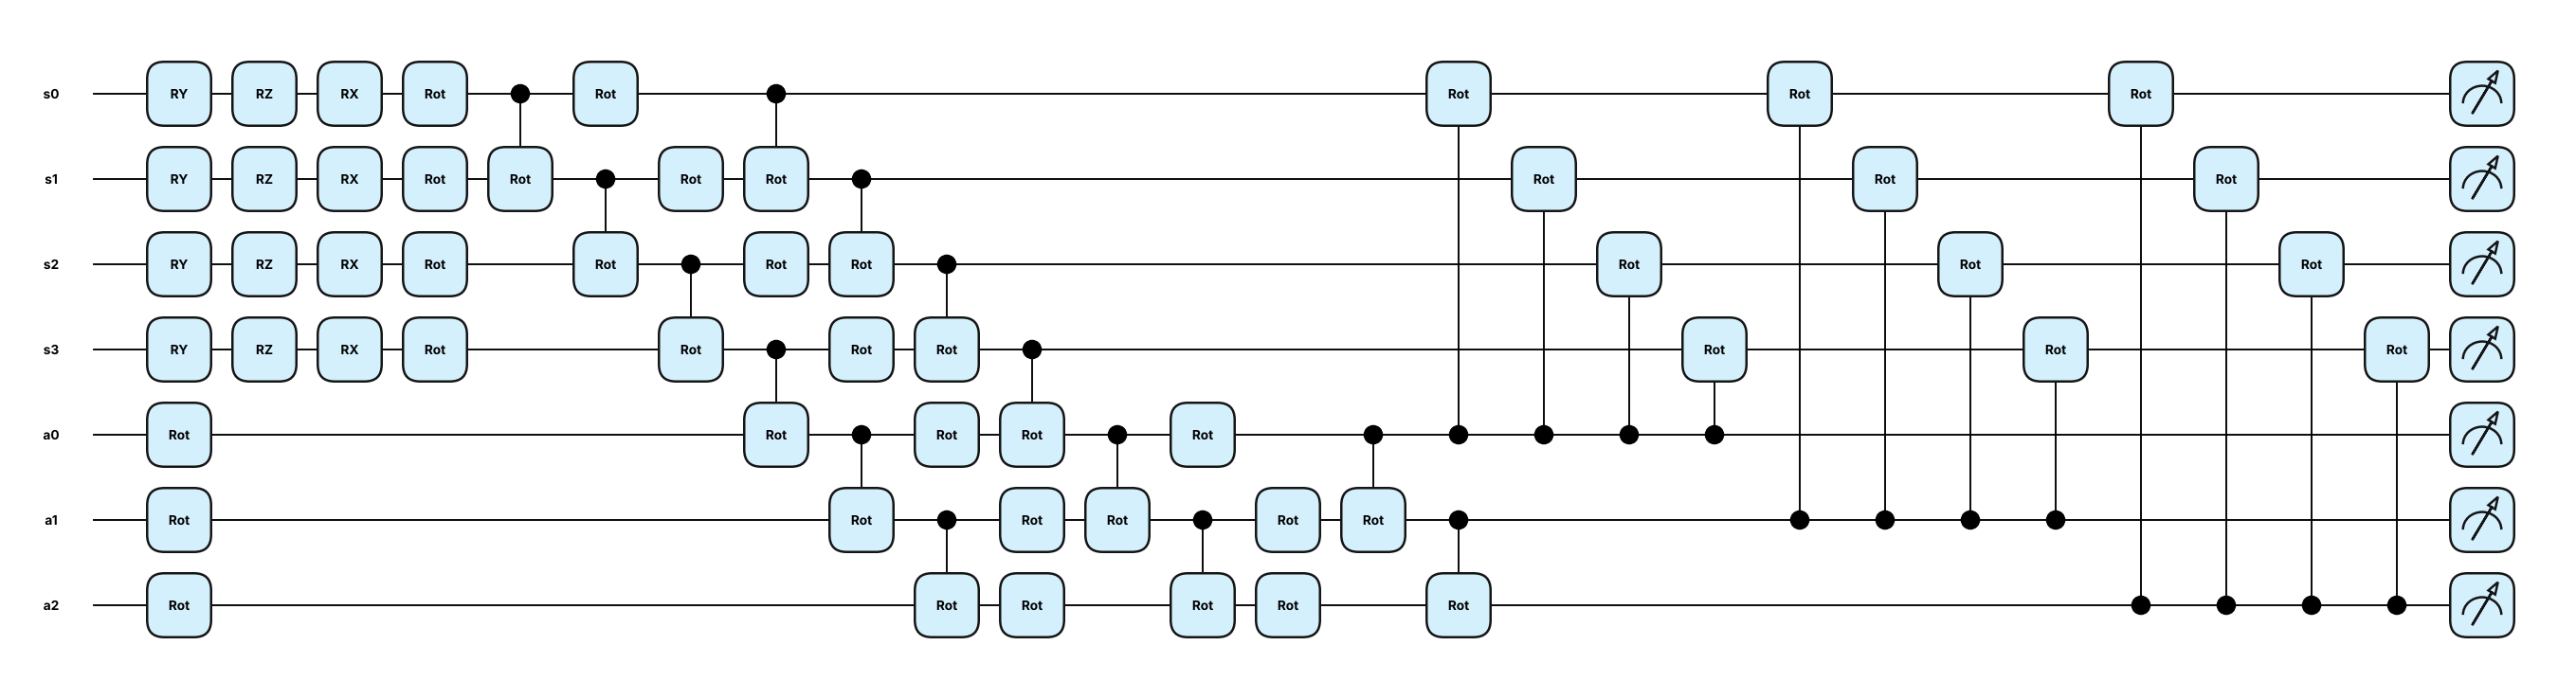
\includegraphics[width=\textwidth]{figures/circuit_one_patch.png}
  \caption{PennyLane drawing of the gates of one patch with $L=2$ repetitions of $W_i$ (the experiments use $L=2$ and $L=4$).}
  \label{fig:onepatch}
\end{figure}

\subsection{MNIST results}

Supplementary Tables~\ref{tab:mnist-results} and~\ref{tab:mnist-amp} give the test accuracies behind Figs.~\ref{fig:capacity} and~\ref{fig:classical}.

\begin{table}[htbp]
  \centering
  \caption{MNIST test accuracy (\%) at the last epoch, mean $\pm$ standard deviation over three seeds. Classical models are sized to the parameter count of the circuit with the given $L$; logistic regression does not depend on $L$. The best mean of each column within each block is in bold. $^\dagger$One of the three seeds stalled at about 47\% training accuracy and is included in the mean. Generated from the result files by \texttt{scripts/paper\_figures.py}.}
  \label{tab:mnist-results}
  \footnotesize
  \setlength{\tabcolsep}{3pt}
  \resizebox{\textwidth}{!}{\input{tables/mnist_results}}
\end{table}

\begin{table}[htbp]
  \centering
  \caption{MNIST test accuracy (\%) of the amplitude-encoding circuits: the whole image as a normalized amplitude vector of 4 qubits (shrunk to $4\times4$) or 7 qubits ($8\times8$ as it is, $14\times14$ shrunk to $11\times11$), followed by $L$ layers of the block of the serialized circuit and the same readout (60--462 parameters). Mean $\pm$ standard deviation over three seeds; the best mean of each column is in bold.}
  \label{tab:mnist-amp}
  \footnotesize
  \setlength{\tabcolsep}{3pt}
  \input{tables/mnist_amplitude}
\end{table}

\subsection{Twelve further datasets}

Supplementary Table~\ref{tab:datasets} describes the datasets and Supplementary Table~\ref{tab:bench} gives the test accuracies behind Fig.~\ref{fig:bench}.

\begin{table}[htbp]
  \centering
  \caption{The twelve further datasets. $d$: features, $N$: patches of four features, $k$: classes. Tabular sets keep their natural class frequencies (majority class in the last column); the image sets are class balanced except PneumoniaMNIST, which keeps its official splits.}
  \label{tab:datasets}
  \footnotesize
  \resizebox{\textwidth}{!}{%
  \begin{tabular}{@{}llrrrrr@{}}
    \toprule
    dataset & source & $d$ & $N$ & $k$ & train / val / test & majority \\
    \midrule
    Waveform & UCI 107~\cite{uci_waveform} (21 wave attributes) & 21 & 6 & 3 & 3\,601 / 400 / 999 & 33.9\% \\
    Wall-Following & UCI 194~\cite{freire2009wall}, 24 sensors & 24 & 6 & 4 & 3\,929 / 436 / 1\,091 & 40.4\% \\
    Covertype & UCI 31~\cite{uci_covertype,blackard1999covertype} & 54 & 14 & 7 & 10\,000 / 2\,000 / 9\,999 & 48.8\% \\
    Letter & UCI 59~\cite{frey1991letter} & 16 & 4 & 26 & 10\,000 / 1\,600 / 4\,000 & 4.1\% \\
    Spambase & UCI 94~\cite{uci_spambase} & 57 & 15 & 2 & 3\,313 / 368 / 920 & 60.5\% \\
    Credit Default & UCI 350~\cite{yeh2009credit} & 23 & 6 & 2 & 10\,000 / 2\,000 / 6\,000 & 77.9\% \\
    Landsat & UCI 146~\cite{uci_landsat,king1995statlog} (train and test joined) & 36 & 9 & 6 & 4\,634 / 514 / 1\,287 & 23.9\% \\
    Dry Bean & UCI 602~\cite{koklu2020drybean} & 16 & 4 & 7 & 9\,801 / 1\,089 / 2\,721 & 26.1\% \\
    \midrule
    Fashion-MNIST & \cite{xiao2017fashion}, $14\times14$ & 196 & 49 & 10 & 10\,000 / 2\,000 / 10\,000 & 10\% \\
    BloodMNIST & MedMNIST v2~\cite{yang2023medmnist,acevedo2020blood}, grayscale, $14\times14$ & 196 & 49 & 8 & 8\,779 / 1\,527 / 3\,421 & 19.5\% \\
    PneumoniaMNIST & MedMNIST v2~\cite{yang2023medmnist,kermany2018pneumonia}, $14\times14$ & 196 & 49 & 2 & 4\,708 / 524 / 624 & 62.5\% \\
    Kuzushiji-MNIST & \cite{clanuwat2018kmnist}, $14\times14$ & 196 & 49 & 10 & 10\,000 / 2\,000 / 10\,000 & 10\% \\
    \bottomrule
  \end{tabular}}
\end{table}

\begin{table}[htbp]
  \centering
  \caption{Test accuracy (\%) on twelve further datasets at the last epoch, mean $\pm$ standard deviation over three seeds; the best mean of each row is in bold. $k$: classes, $N$: patches of four features, params: parameters of the circuit with coherent memory and $L=4$, which is also the size of the MLP and the CNN. Amplitude: the whole input as the amplitude vector of the same seven qubits with $L=4$ or $8$ layers of the same block (200--550 parameters). Gradient boosting: scikit-learn histogram gradient boosting, an ensemble of 300 trees shown as a reference, not tuned. Measured memory was run on the tabular sets only (above the line).}
  \label{tab:bench}
  \footnotesize
  \setlength{\tabcolsep}{2.5pt}
  \resizebox{\textwidth}{!}{\input{tables/bench_results}}
\end{table}

\begin{table}[htbp]
  \centering
  \caption{As Supplementary Table~\ref{tab:bench}, but balanced accuracy (\%), the mean of the per-class recalls: last epoch, mean $\pm$ standard deviation over three seeds; the best mean of each row is in bold.}
  \label{tab:bench-bal}
  \footnotesize
  \setlength{\tabcolsep}{2.5pt}
  \resizebox{\textwidth}{!}{\input{tables/bench_balanced}}
\end{table}

\subsection{Classical models with the structure of the circuit}

\begin{table}[htbp]
  \centering
  \caption{The serialized circuit ($L=4$) against classical models that read the input patch by patch with position-specific parameters. Test accuracy (\%) at the last epoch, mean over three seeds; the best mean of each row is in bold. MLP: the one-hidden-layer MLP of Supplementary Table~\ref{tab:bench} (for MNIST, the parameter-matched MLP of Supplementary Table~\ref{tab:mnist-results}). Seq.\ RNN: recurrent network with its own weights at every patch; MPS: matrix-product-state classifier with one tensor per feature; both are sized to the parameter count of the circuit as closely as their hidden or bond dimension allows. 8-state HMM: input-driven hidden Markov model over eight states, with 1.5 to 2 times the parameters of the circuit. The learning rate of each classical model is chosen by mean validation accuracy. Measured memory was not run on the 49-patch image sets.}
  \label{tab:struct}
  \footnotesize
  \input{tables/struct_baselines}
\end{table}

\subsection{Readout and head variants on Letter}

Supplementary Table~\ref{tab:letter} collects the variants of the circuit run on Letter, each against a one-hidden-layer MLP with the same number of parameters.

\begin{table}[htbp]
  \centering
  \caption{Letter (26 classes): readout, head and depth variants of the circuit with coherent memory, against a one-hidden-layer MLP of the same size. Test accuracy (\%), mean $\pm$ standard deviation over three seeds; the better mean of each row is in bold. Gradient-boosted trees reach $95.3\pm0.1$.}
  \label{tab:letter}
  \footnotesize
  \input{tables/letter_variants}
\end{table}

\subsection{$28\times28$ images}
\label{sec:supp-28}

At $28\times28$ the serialized circuit has 196 patches and 74\% of them are empty (62\% at $14\times14$, 41\% at $8\times8$). With the settings of the MNIST experiments it stays at chance or only fits the training set, and the simulation takes about 47 minutes (3 vs.\ 5) to 2 hours (10 classes) per epoch, i.e.\ days per run, so it is not reported. The classical and amplitude-encoding baselines were run at $28\times28$ and are in the code repository.
 after \appendix.
\section{Supplementary Information}
\label{sec:supp}
\renewcommand{\thefigure}{S\arabic{figure}}
\renewcommand{\thetable}{S\arabic{table}}
\setcounter{figure}{0}
\setcounter{table}{0}

\subsection{Gates of one patch}

Supplementary Fig.~\ref{fig:onepatch} shows the gates acting on one patch, as drawn by PennyLane for $L=2$: the encoding rotations on the system qubits, the $\mathrm{Rot}$ layers and $\mathrm{CRot}$ chains of $W_i$, and $W_c$ with the controlled rotations from each ancilla to the system qubits.

\begin{figure}[h]
  \centering
  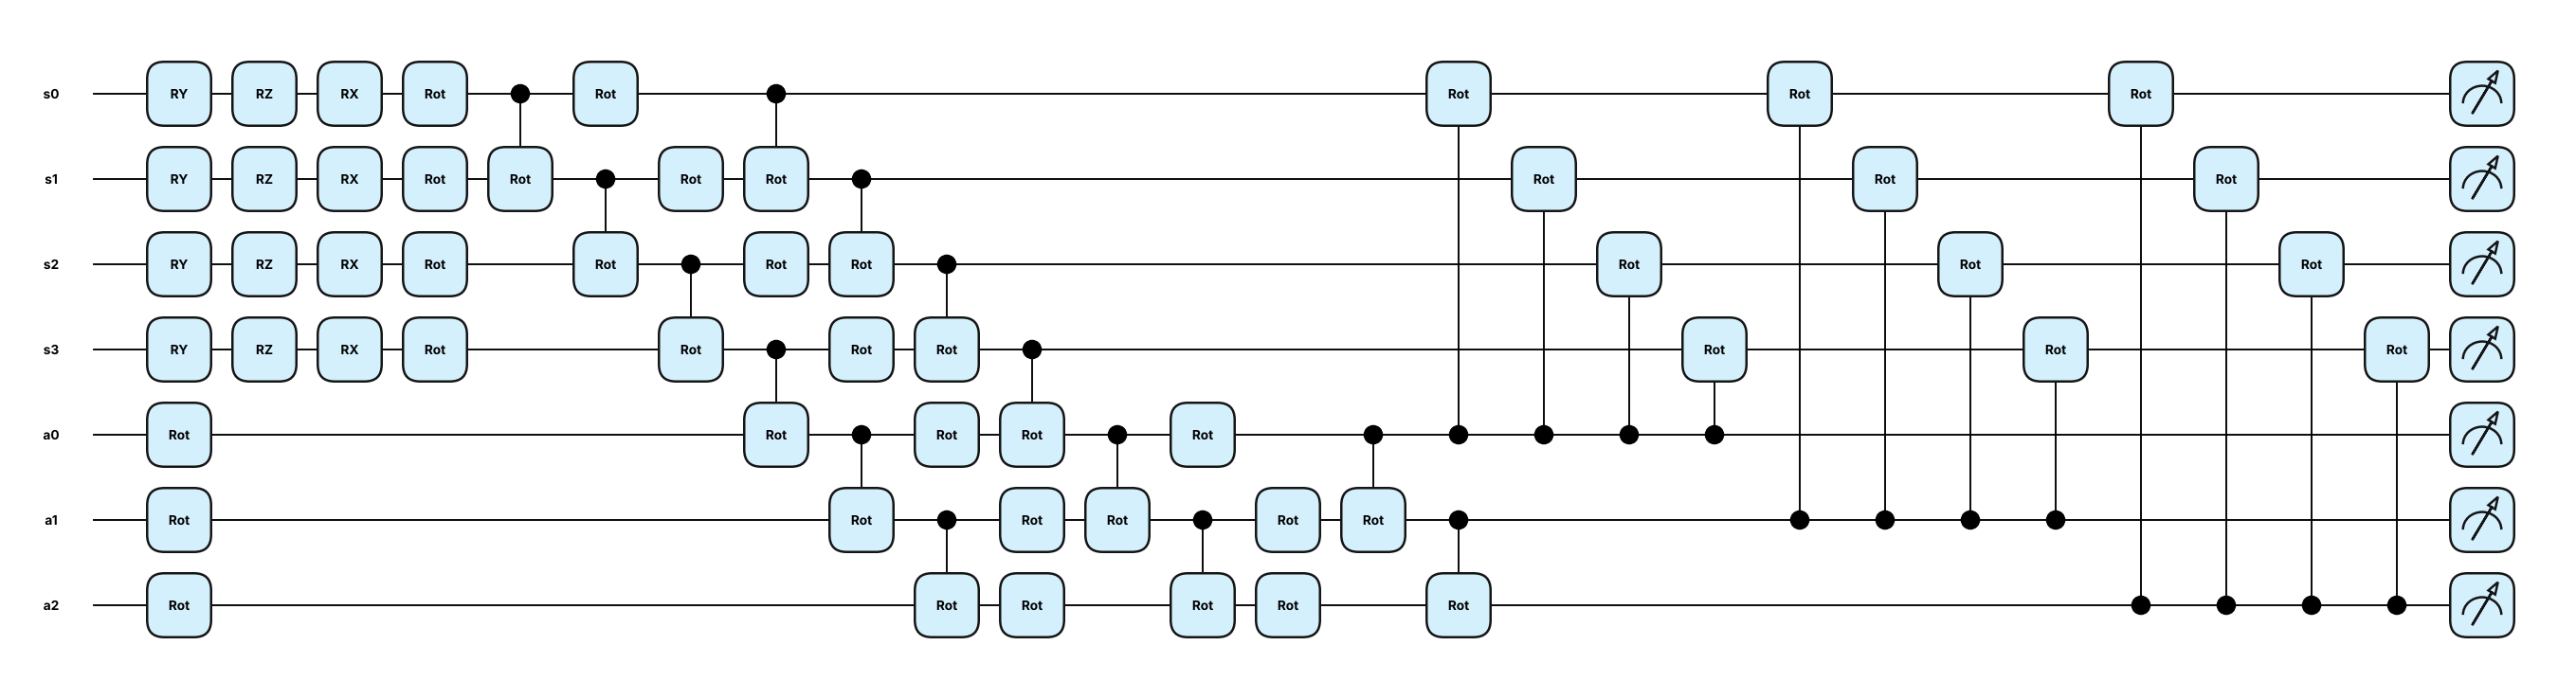
\includegraphics[width=\textwidth]{figures/circuit_one_patch.png}
  \caption{PennyLane drawing of the gates of one patch with $L=2$ repetitions of $W_i$ (the experiments use $L=2$ and $L=4$).}
  \label{fig:onepatch}
\end{figure}

\subsection{MNIST results}

Supplementary Tables~\ref{tab:mnist-results} and~\ref{tab:mnist-amp} give the test accuracies behind Figs.~\ref{fig:capacity} and~\ref{fig:classical}.

\begin{table}[htbp]
  \centering
  \caption{MNIST test accuracy (\%) at the last epoch, mean $\pm$ standard deviation over three seeds. Classical models are sized to the parameter count of the circuit with the given $L$; logistic regression does not depend on $L$. The best mean of each column within each block is in bold. $^\dagger$One of the three seeds stalled at about 47\% training accuracy and is included in the mean. Generated from the result files by \texttt{scripts/paper\_figures.py}.}
  \label{tab:mnist-results}
  \footnotesize
  \setlength{\tabcolsep}{3pt}
  \resizebox{\textwidth}{!}{% generated by scripts/paper_figures.py -- do not edit
\begin{tabular}{@{}lcccccccc@{}}
\toprule
 & \multicolumn{2}{c}{3 vs 5} & \multicolumn{2}{c}{4 vs 9} & \multicolumn{2}{c}{4 classes (0-3)} & \multicolumn{2}{c}{10 classes} \\
\cmidrule(lr){2-3}\cmidrule(lr){4-5}\cmidrule(lr){6-7}\cmidrule(lr){8-9}
 & $8{\times}8$ & $14{\times}14$ & $8{\times}8$ & $14{\times}14$ & $8{\times}8$ & $14{\times}14$ & $8{\times}8$ & $14{\times}14$ \\
\midrule
\multicolumn{9}{@{}l}{\emph{$L=2$ (classical models sized to the circuit with $L=2$)}} \\
serialized, coherent & $96.2\pm0.5$ & $96.9\pm0.2$ & $94.3\pm0.3$ & $96.3\pm0.5$ & $97.4\pm0.2$ & $97.7\pm0.2$ & $89.9\pm0.1$ & $91.8\pm0.2$ \\
serialized, measured & $95.7\pm0.5$ & $96.8\pm0.6$ & $92.6\pm0.4$ & $96.1\pm0.3$ & $90.7\pm4.8$ & $97.0\pm0.1$ & $64.0\pm14.1$$^\dagger$ & $79.9\pm2.8$ \\
MLP, same parameters & $95.6\pm0.1$ & $97.2\pm1.5$ & $95.8\pm0.1$ & $97.3\pm0.6$ & $97.7\pm0.3$ & $98.0\pm0.1$ & $92.0\pm0.2$ & $93.7\pm0.3$ \\
CNN, same parameters & $\mathbf{98.2}\pm0.2$ & $\mathbf{98.5}\pm0.3$ & $\mathbf{96.4}\pm0.2$ & $\mathbf{98.7}\pm0.2$ & $\mathbf{98.7}\pm0.1$ & $\mathbf{99.0}\pm0.1$ & $\mathbf{93.6}\pm0.5$ & $\mathbf{96.3}\pm0.1$ \\
logistic regression & $95.1\pm0.2$ & $95.7\pm0.5$ & $94.8\pm0.2$ & $97.0\pm0.3$ & $97.1\pm0.1$ & $97.5\pm0.1$ & $89.9\pm0.1$ & $91.7\pm0.1$ \\
\midrule
\multicolumn{9}{@{}l}{\emph{$L=4$ (classical models sized to the circuit with $L=4$)}} \\
serialized, coherent & $97.2\pm0.3$ & $97.5\pm0.2$ & $94.9\pm0.3$ & $97.0\pm0.6$ & $97.0\pm0.1$ & $97.8\pm0.3$ & $91.1\pm0.3$ & $92.8\pm0.4$ \\
serialized, measured & $96.9\pm0.2$ & $97.0\pm0.6$ & $94.8\pm0.4$ & $96.8\pm0.3$ & $96.3\pm0.6$ & $97.5\pm0.2$ & $81.2\pm4.1$ & $86.2\pm3.3$ \\
MLP, same parameters & $97.7\pm0.7$ & $98.0\pm0.6$ & $96.8\pm0.3$ & $97.7\pm0.4$ & $98.3\pm0.2$ & $98.3\pm0.0$ & $94.7\pm0.3$ & $95.1\pm0.1$ \\
CNN, same parameters & $\mathbf{98.4}\pm0.4$ & $\mathbf{98.7}\pm0.1$ & $\mathbf{97.0}\pm0.4$ & $\mathbf{98.9}\pm0.2$ & $\mathbf{98.8}\pm0.0$ & $\mathbf{99.1}\pm0.1$ & $\mathbf{95.3}\pm0.2$ & $\mathbf{97.2}\pm0.2$ \\
\bottomrule
\end{tabular}
}
\end{table}

\begin{table}[htbp]
  \centering
  \caption{MNIST test accuracy (\%) of the amplitude-encoding circuits: the whole image as a normalized amplitude vector of 4 qubits (shrunk to $4\times4$) or 7 qubits ($8\times8$ as it is, $14\times14$ shrunk to $11\times11$), followed by $L$ layers of the block of the serialized circuit and the same readout (60--462 parameters). Mean $\pm$ standard deviation over three seeds; the best mean of each column is in bold.}
  \label{tab:mnist-amp}
  \footnotesize
  \setlength{\tabcolsep}{3pt}
  % generated by scripts/paper_figures.py -- do not edit
\begin{tabular}{@{}llcccccccc@{}}
\toprule
 & & \multicolumn{2}{c}{3 vs 5} & \multicolumn{2}{c}{4 vs 9} & \multicolumn{2}{c}{4 classes (0-3)} & \multicolumn{2}{c}{10 classes} \\
\cmidrule(lr){3-4}\cmidrule(lr){5-6}\cmidrule(lr){7-8}\cmidrule(lr){9-10}
qubits & $L$ & $8{\times}8$ & $14{\times}14$ & $8{\times}8$ & $14{\times}14$ & $8{\times}8$ & $14{\times}14$ & $8{\times}8$ & $14{\times}14$ \\
\midrule
4 & 2 & $93.6\pm0.7$ & $93.8\pm0.4$ & $78.0\pm0.6$ & $83.5\pm0.3$ & $88.7\pm0.1$ & $89.2\pm1.1$ & $68.8\pm0.1$ & $72.1\pm1.4$ \\
4 & 4 & $93.9\pm0.2$ & $94.6\pm0.2$ & $79.0\pm1.8$ & $85.0\pm0.4$ & $89.1\pm0.3$ & $90.6\pm0.1$ & $70.5\pm0.7$ & $75.6\pm0.6$ \\
4 & 8 & $94.4\pm0.4$ & $94.6\pm0.2$ & $79.7\pm0.5$ & $85.3\pm1.0$ & $90.0\pm0.4$ & $90.9\pm0.4$ & $72.4\pm0.3$ & $76.4\pm0.9$ \\
\midrule
7 & 2 & $93.5\pm1.4$ & $92.3\pm0.2$ & $88.4\pm0.4$ & $94.9\pm0.4$ & $96.0\pm0.2$ & $96.0\pm0.1$ & $82.4\pm1.2$ & $82.9\pm1.5$ \\
7 & 4 & $94.9\pm1.0$ & $94.6\pm0.8$ & $90.2\pm0.1$ & $\mathbf{95.2}\pm0.1$ & $96.6\pm0.4$ & $96.8\pm0.4$ & $86.3\pm0.2$ & $86.4\pm1.0$ \\
7 & 8 & $\mathbf{96.0}\pm0.5$ & $\mathbf{95.7}\pm0.5$ & $\mathbf{93.5}\pm0.6$ & $\mathbf{95.2}\pm0.5$ & $\mathbf{97.5}\pm0.2$ & $\mathbf{97.1}\pm0.2$ & $\mathbf{87.9}\pm0.4$ & $\mathbf{89.2}\pm0.5$ \\
\bottomrule
\end{tabular}

\end{table}

\subsection{Twelve further datasets}

Supplementary Table~\ref{tab:datasets} describes the datasets and Supplementary Table~\ref{tab:bench} gives the test accuracies behind Fig.~\ref{fig:bench}.

\begin{table}[htbp]
  \centering
  \caption{The twelve further datasets. $d$: features, $N$: patches of four features, $k$: classes. Tabular sets keep their natural class frequencies (majority class in the last column); the image sets are class balanced except PneumoniaMNIST, which keeps its official splits.}
  \label{tab:datasets}
  \footnotesize
  \resizebox{\textwidth}{!}{%
  \begin{tabular}{@{}llrrrrr@{}}
    \toprule
    dataset & source & $d$ & $N$ & $k$ & train / val / test & majority \\
    \midrule
    Waveform & UCI 107~\cite{uci_waveform} (21 wave attributes) & 21 & 6 & 3 & 3\,601 / 400 / 999 & 33.9\% \\
    Wall-Following & UCI 194~\cite{freire2009wall}, 24 sensors & 24 & 6 & 4 & 3\,929 / 436 / 1\,091 & 40.4\% \\
    Covertype & UCI 31~\cite{uci_covertype,blackard1999covertype} & 54 & 14 & 7 & 10\,000 / 2\,000 / 9\,999 & 48.8\% \\
    Letter & UCI 59~\cite{frey1991letter} & 16 & 4 & 26 & 10\,000 / 1\,600 / 4\,000 & 4.1\% \\
    Spambase & UCI 94~\cite{uci_spambase} & 57 & 15 & 2 & 3\,313 / 368 / 920 & 60.5\% \\
    Credit Default & UCI 350~\cite{yeh2009credit} & 23 & 6 & 2 & 10\,000 / 2\,000 / 6\,000 & 77.9\% \\
    Landsat & UCI 146~\cite{uci_landsat,king1995statlog} (train and test joined) & 36 & 9 & 6 & 4\,634 / 514 / 1\,287 & 23.9\% \\
    Dry Bean & UCI 602~\cite{koklu2020drybean} & 16 & 4 & 7 & 9\,801 / 1\,089 / 2\,721 & 26.1\% \\
    \midrule
    Fashion-MNIST & \cite{xiao2017fashion}, $14\times14$ & 196 & 49 & 10 & 10\,000 / 2\,000 / 10\,000 & 10\% \\
    BloodMNIST & MedMNIST v2~\cite{yang2023medmnist,acevedo2020blood}, grayscale, $14\times14$ & 196 & 49 & 8 & 8\,779 / 1\,527 / 3\,421 & 19.5\% \\
    PneumoniaMNIST & MedMNIST v2~\cite{yang2023medmnist,kermany2018pneumonia}, $14\times14$ & 196 & 49 & 2 & 4\,708 / 524 / 624 & 62.5\% \\
    Kuzushiji-MNIST & \cite{clanuwat2018kmnist}, $14\times14$ & 196 & 49 & 10 & 10\,000 / 2\,000 / 10\,000 & 10\% \\
    \bottomrule
  \end{tabular}}
\end{table}

\begin{table}[htbp]
  \centering
  \caption{Test accuracy (\%) on twelve further datasets at the last epoch, mean $\pm$ standard deviation over three seeds; the best mean of each row is in bold. $k$: classes, $N$: patches of four features, params: parameters of the circuit with coherent memory and $L=4$, which is also the size of the MLP and the CNN. Amplitude: the whole input as the amplitude vector of the same seven qubits with $L=4$ or $8$ layers of the same block (200--550 parameters). Gradient boosting: scikit-learn histogram gradient boosting, an ensemble of 300 trees shown as a reference, not tuned. Measured memory was run on the tabular sets only (above the line).}
  \label{tab:bench}
  \footnotesize
  \setlength{\tabcolsep}{2.5pt}
  \resizebox{\textwidth}{!}{% generated by scripts/paper_figures.py -- do not edit
\begin{tabular}{@{}lrrrrrrrrrrr@{}}
\toprule
 & & & & \multicolumn{4}{c}{classical} & \multicolumn{2}{c}{amplitude, 7 qubits} & \multicolumn{2}{c@{}}{serialized, 7 qubits} \\
\cmidrule(lr){5-8}\cmidrule(lr){9-10}\cmidrule(l){11-12}
dataset & $k$ & $N$ & params & logistic & MLP & CNN & grad.\ boost. & $L{=}4$ & $L{=}8$ & \multicolumn{1}{c}{coherent} & \multicolumn{1}{c@{}}{measured} \\
\midrule
Waveform & 3 & 6 & 1056 & $\mathbf{87.2}${\scriptsize$\pm0.1$} & $87.1${\scriptsize$\pm0.8$} & -- & $85.5${\scriptsize$\pm0.5$} & $86.2${\scriptsize$\pm0.2$} & $86.8${\scriptsize$\pm0.6$} & $85.0${\scriptsize$\pm0.2$} & $82.7${\scriptsize$\pm3.1$} \\
Wall-Following & 4 & 6 & 1071 & $68.3${\scriptsize$\pm0.3$} & $91.9${\scriptsize$\pm0.4$} & -- & $\mathbf{99.9}${\scriptsize$\pm0.0$} & $73.0${\scriptsize$\pm1.4$} & $77.1${\scriptsize$\pm1.5$} & $90.1${\scriptsize$\pm0.7$} & $87.0${\scriptsize$\pm2.0$} \\
Covertype & 7 & 14 & 2364 & $71.6${\scriptsize$\pm0.1$} & $75.8${\scriptsize$\pm0.2$} & -- & $\mathbf{82.2}${\scriptsize$\pm0.2$} & $71.7${\scriptsize$\pm0.5$} & $72.0${\scriptsize$\pm0.3$} & $73.8${\scriptsize$\pm0.2$} & $71.7${\scriptsize$\pm0.5$} \\
Letter & 26 & 4 & 1089 & $72.6${\scriptsize$\pm0.2$} & $80.4${\scriptsize$\pm0.8$} & -- & $\mathbf{95.3}${\scriptsize$\pm0.1$} & $59.7${\scriptsize$\pm2.5$} & $63.6${\scriptsize$\pm0.8$} & $71.0${\scriptsize$\pm1.6$} & $63.5${\scriptsize$\pm3.1$} \\
Spambase & 2 & 15 & 2445 & $92.0${\scriptsize$\pm0.1$} & $93.4${\scriptsize$\pm0.5$} & -- & $\mathbf{96.1}${\scriptsize$\pm0.3$} & $90.0${\scriptsize$\pm0.4$} & $90.7${\scriptsize$\pm0.8$} & $91.7${\scriptsize$\pm0.4$} & $93.5${\scriptsize$\pm0.6$} \\
Credit Default & 2 & 6 & 1041 & $81.1${\scriptsize$\pm0.1$} & $81.7${\scriptsize$\pm0.1$} & -- & $81.4${\scriptsize$\pm0.3$} & $79.6${\scriptsize$\pm0.2$} & $79.7${\scriptsize$\pm0.1$} & $81.9${\scriptsize$\pm0.3$} & $\mathbf{82.4}${\scriptsize$\pm0.1$} \\
Landsat & 6 & 9 & 1569 & $82.3${\scriptsize$\pm0.2$} & $89.2${\scriptsize$\pm0.1$} & -- & $\mathbf{92.3}${\scriptsize$\pm0.5$} & $78.7${\scriptsize$\pm0.2$} & $78.9${\scriptsize$\pm0.2$} & $89.3${\scriptsize$\pm1.2$} & $86.8${\scriptsize$\pm1.0$} \\
Dry Bean & 7 & 4 & 804 & $92.1${\scriptsize$\pm0.0$} & $92.3${\scriptsize$\pm0.1$} & -- & $92.8${\scriptsize$\pm0.2$} & $91.8${\scriptsize$\pm0.1$} & $91.8${\scriptsize$\pm0.2$} & $\mathbf{92.9}${\scriptsize$\pm0.2$} & $92.8${\scriptsize$\pm0.0$} \\
\midrule
Fashion-MNIST & 10 & 49 & 7869 & $82.6${\scriptsize$\pm0.2$} & $85.2${\scriptsize$\pm0.1$} & $85.7${\scriptsize$\pm0.6$} & $\mathbf{86.5}${\scriptsize$\pm0.4$} & $73.7${\scriptsize$\pm0.4$} & $74.4${\scriptsize$\pm0.8$} & $82.7${\scriptsize$\pm0.2$} & -- \\
BloodMNIST & 8 & 49 & 7839 & $67.2${\scriptsize$\pm0.4$} & $70.3${\scriptsize$\pm1.2$} & $81.2${\scriptsize$\pm0.4$} & $\mathbf{86.0}${\scriptsize$\pm0.2$} & $58.0${\scriptsize$\pm0.6$} & $60.2${\scriptsize$\pm0.2$} & $73.8${\scriptsize$\pm1.3$} & -- \\
PneumoniaMNIST & 2 & 49 & 7749 & $83.5${\scriptsize$\pm0.1$} & $84.1${\scriptsize$\pm0.9$} & $85.6${\scriptsize$\pm0.8$} & $84.9${\scriptsize$\pm0.0$} & $81.2${\scriptsize$\pm1.5$} & $81.9${\scriptsize$\pm1.2$} & $\mathbf{87.7}${\scriptsize$\pm0.7$} & -- \\
Kuzushiji-MNIST & 10 & 49 & 7869 & $68.2${\scriptsize$\pm0.3$} & $78.7${\scriptsize$\pm0.2$} & $80.3${\scriptsize$\pm1.5$} & $\mathbf{83.4}${\scriptsize$\pm0.3$} & $58.3${\scriptsize$\pm0.8$} & $62.6${\scriptsize$\pm0.8$} & $70.4${\scriptsize$\pm0.7$} & -- \\
\bottomrule
\end{tabular}
}
\end{table}

\begin{table}[htbp]
  \centering
  \caption{As Supplementary Table~\ref{tab:bench}, but balanced accuracy (\%), the mean of the per-class recalls: last epoch, mean $\pm$ standard deviation over three seeds; the best mean of each row is in bold.}
  \label{tab:bench-bal}
  \footnotesize
  \setlength{\tabcolsep}{2.5pt}
  \resizebox{\textwidth}{!}{% generated by scripts/paper_figures.py -- do not edit
\begin{tabular}{@{}lrrrrrrrrrrr@{}}
\toprule
 & & & & \multicolumn{4}{c}{classical} & \multicolumn{2}{c}{amplitude, 7 qubits} & \multicolumn{2}{c@{}}{serialized, 7 qubits} \\
\cmidrule(lr){5-8}\cmidrule(lr){9-10}\cmidrule(l){11-12}
dataset & $k$ & $N$ & params & logistic & MLP & CNN & grad.\ boost. & $L{=}4$ & $L{=}8$ & \multicolumn{1}{c}{coherent} & \multicolumn{1}{c@{}}{measured} \\
\midrule
Waveform & 3 & 6 & 1056 & $\mathbf{87.2}${\scriptsize$\pm0.1$} & $87.1${\scriptsize$\pm0.8$} & -- & $85.5${\scriptsize$\pm0.5$} & $86.2${\scriptsize$\pm0.2$} & $86.8${\scriptsize$\pm0.6$} & $85.0${\scriptsize$\pm0.2$} & $82.7${\scriptsize$\pm3.1$} \\
Wall-Following & 4 & 6 & 1071 & $59.7${\scriptsize$\pm1.0$} & $90.8${\scriptsize$\pm0.9$} & -- & $\mathbf{99.9}${\scriptsize$\pm0.0$} & $66.2${\scriptsize$\pm1.8$} & $69.9${\scriptsize$\pm0.9$} & $88.8${\scriptsize$\pm0.8$} & $84.6${\scriptsize$\pm2.7$} \\
Covertype & 7 & 14 & 2364 & $46.0${\scriptsize$\pm1.2$} & $56.2${\scriptsize$\pm2.4$} & -- & $\mathbf{67.8}${\scriptsize$\pm0.2$} & $42.3${\scriptsize$\pm0.1$} & $42.1${\scriptsize$\pm1.7$} & $45.3${\scriptsize$\pm1.2$} & $38.1${\scriptsize$\pm2.6$} \\
Letter & 26 & 4 & 1089 & $72.5${\scriptsize$\pm0.2$} & $80.4${\scriptsize$\pm0.8$} & -- & $\mathbf{95.3}${\scriptsize$\pm0.1$} & $59.6${\scriptsize$\pm2.4$} & $63.5${\scriptsize$\pm0.7$} & $70.8${\scriptsize$\pm1.6$} & $63.5${\scriptsize$\pm3.1$} \\
Spambase & 2 & 15 & 2445 & $91.2${\scriptsize$\pm0.1$} & $92.9${\scriptsize$\pm0.4$} & -- & $\mathbf{96.1}${\scriptsize$\pm0.3$} & $89.2${\scriptsize$\pm0.5$} & $90.0${\scriptsize$\pm0.8$} & $91.4${\scriptsize$\pm0.8$} & $93.1${\scriptsize$\pm0.7$} \\
Credit Default & 2 & 6 & 1041 & $61.2${\scriptsize$\pm0.2$} & $65.4${\scriptsize$\pm0.3$} & -- & $65.0${\scriptsize$\pm0.2$} & $58.5${\scriptsize$\pm0.4$} & $59.1${\scriptsize$\pm0.3$} & $65.3${\scriptsize$\pm0.7$} & $\mathbf{66.3}${\scriptsize$\pm0.4$} \\
Landsat & 6 & 9 & 1569 & $74.7${\scriptsize$\pm0.4$} & $86.5${\scriptsize$\pm0.1$} & -- & $\mathbf{90.1}${\scriptsize$\pm0.6$} & $69.3${\scriptsize$\pm0.2$} & $69.4${\scriptsize$\pm0.2$} & $86.8${\scriptsize$\pm1.4$} & $83.6${\scriptsize$\pm1.3$} \\
Dry Bean & 7 & 4 & 804 & $93.4${\scriptsize$\pm0.0$} & $93.5${\scriptsize$\pm0.0$} & -- & $93.8${\scriptsize$\pm0.2$} & $92.9${\scriptsize$\pm0.2$} & $93.0${\scriptsize$\pm0.1$} & $\mathbf{93.9}${\scriptsize$\pm0.2$} & $93.8${\scriptsize$\pm0.1$} \\
\midrule
Fashion-MNIST & 10 & 49 & 7869 & $82.6${\scriptsize$\pm0.2$} & $85.2${\scriptsize$\pm0.1$} & $85.7${\scriptsize$\pm0.6$} & $\mathbf{86.5}${\scriptsize$\pm0.4$} & $73.7${\scriptsize$\pm0.4$} & $74.4${\scriptsize$\pm0.8$} & $82.7${\scriptsize$\pm0.2$} & -- \\
BloodMNIST & 8 & 49 & 7839 & $67.2${\scriptsize$\pm0.4$} & $69.8${\scriptsize$\pm1.1$} & $79.5${\scriptsize$\pm0.4$} & $\mathbf{84.8}${\scriptsize$\pm0.3$} & $55.5${\scriptsize$\pm0.5$} & $57.4${\scriptsize$\pm1.1$} & $73.0${\scriptsize$\pm1.1$} & -- \\
PneumoniaMNIST & 2 & 49 & 7749 & $78.9${\scriptsize$\pm0.2$} & $79.3${\scriptsize$\pm1.4$} & $81.2${\scriptsize$\pm1.2$} & $80.8${\scriptsize$\pm0.0$} & $76.1${\scriptsize$\pm2.1$} & $77.0${\scriptsize$\pm1.8$} & $\mathbf{84.0}${\scriptsize$\pm1.0$} & -- \\
Kuzushiji-MNIST & 10 & 49 & 7869 & $68.2${\scriptsize$\pm0.3$} & $78.7${\scriptsize$\pm0.2$} & $80.3${\scriptsize$\pm1.5$} & $\mathbf{83.4}${\scriptsize$\pm0.3$} & $58.3${\scriptsize$\pm0.8$} & $62.6${\scriptsize$\pm0.8$} & $70.4${\scriptsize$\pm0.7$} & -- \\
\bottomrule
\end{tabular}
}
\end{table}

\subsection{Classical models with the structure of the circuit}

\begin{table}[htbp]
  \centering
  \caption{The serialized circuit ($L=4$) against classical models that read the input patch by patch with position-specific parameters. Test accuracy (\%) at the last epoch, mean over three seeds; the best mean of each row is in bold. MLP: the one-hidden-layer MLP of Supplementary Table~\ref{tab:bench} (for MNIST, the parameter-matched MLP of Supplementary Table~\ref{tab:mnist-results}). Seq.\ RNN: recurrent network with its own weights at every patch; MPS: matrix-product-state classifier with one tensor per feature; both are sized to the parameter count of the circuit as closely as their hidden or bond dimension allows. 8-state HMM: input-driven hidden Markov model over eight states, with 1.5 to 2 times the parameters of the circuit. The learning rate of each classical model is chosen by mean validation accuracy. Measured memory was not run on the 49-patch image sets.}
  \label{tab:struct}
  \footnotesize
  % generated by scripts/paper_figures.py -- do not edit
\begin{tabular}{@{}lrrrrrr@{}}
\toprule
 & \multicolumn{2}{c}{serialized circuit} & \multicolumn{4}{c@{}}{classical} \\
\cmidrule(lr){2-3}\cmidrule(l){4-7}
dataset & coherent & measured & MLP & seq.\ RNN & MPS & 8-state HMM \\
\midrule
Waveform & $85.0$ & $82.7$ & $87.1$ & $87.4$ & $\mathbf{87.5}$ & $84.9$ \\
Wall-Following & $90.1$ & $87.0$ & $91.9$ & $93.1$ & $\mathbf{95.2}$ & $85.7$ \\
Covertype & $73.8$ & $71.7$ & $\mathbf{75.8}$ & $75.3$ & $75.2$ & $71.3$ \\
Letter & $71.0$ & $63.5$ & $80.4$ & $\mathbf{80.7}$ & $71.4$ & $53.8$ \\
Spambase & $91.7$ & $93.5$ & $93.4$ & $93.2$ & $\mathbf{93.8}$ & $92.5$ \\
Credit Default & $81.9$ & $\mathbf{82.4}$ & $81.7$ & $82.2$ & $82.0$ & $81.9$ \\
Landsat & $89.3$ & $86.8$ & $89.2$ & $\mathbf{89.7}$ & $89.6$ & $83.7$ \\
Dry Bean & $\mathbf{92.9}$ & $92.8$ & $92.3$ & $92.8$ & $\mathbf{92.9}$ & $91.9$ \\
Fashion-MNIST & $82.7$ & -- & $\mathbf{85.2}$ & $77.1$ & $82.2$ & $53.0$ \\
BloodMNIST & $\mathbf{73.8}$ & -- & $70.3$ & $64.7$ & $71.9$ & $44.9$ \\
PneumoniaMNIST & $\mathbf{87.7}$ & -- & $84.1$ & $87.6$ & $87.5$ & $82.9$ \\
Kuzushiji-MNIST & $70.4$ & -- & $\mathbf{78.7}$ & $61.8$ & $62.1$ & $31.0$ \\
MNIST $8\times8$, 3 vs.\ 5 & $97.2$ & $96.9$ & $97.7$ & $\mathbf{98.1}$ & $97.4$ & $65.0$ \\
MNIST $8\times8$, 10 classes & $91.1$ & $81.2$ & $\mathbf{94.7}$ & $92.7$ & $92.1$ & $68.2$ \\
\bottomrule
\end{tabular}

\end{table}

\subsection{Readout and head variants on Letter}

Supplementary Table~\ref{tab:letter} collects the variants of the circuit run on Letter, each against a one-hidden-layer MLP with the same number of parameters.

\begin{table}[htbp]
  \centering
  \caption{Letter (26 classes): readout, head and depth variants of the circuit with coherent memory, against a one-hidden-layer MLP of the same size. Test accuracy (\%), mean $\pm$ standard deviation over three seeds; the better mean of each row is in bold. Gradient-boosted trees reach $95.3\pm0.1$.}
  \label{tab:letter}
  \footnotesize
  % generated by scripts/paper_figures.py -- do not edit
\begin{tabular}{@{}lrlrl@{}}
\toprule
 & \multicolumn{2}{c}{circuit} & \multicolumn{2}{c@{}}{MLP, same size} \\
\cmidrule(lr){2-3}\cmidrule(l){4-5}
readout and head & params & accuracy & params & accuracy \\
\midrule
$Z$, $ZZ$ (14 features), linear head, $L=4$ & 1\,089 & $71.0\pm1.6$ & 1\,101 & $\mathbf{80.4}\pm0.8$ \\
$Z$, $ZZ$ (14 features), linear head, $L=9$ & 1\,869 & $71.8\pm2.1$ & -- & -- \\
$+X$, $XX$, $Y$, $YY$ (42 features), linear head, $L=4$ & 1\,817 & $79.9\pm0.2$ & 1\,832 & $\mathbf{84.7}\pm1.2$ \\
$Z$, $ZZ$ (14 features), MLP head (64 units), $L=4$ & 3\,349 & $85.6\pm0.6$ & 3\,337 & $\mathbf{87.8}\pm0.2$ \\
\bottomrule
\end{tabular}

\end{table}

\subsection{$28\times28$ images}
\label{sec:supp-28}

At $28\times28$ the serialized circuit has 196 patches and 74\% of them are empty (62\% at $14\times14$, 41\% at $8\times8$). With the settings of the MNIST experiments it stays at chance or only fits the training set, and the simulation takes about 47 minutes (3 vs.\ 5) to 2 hours (10 classes) per epoch, i.e.\ days per run, so it is not reported. The classical and amplitude-encoding baselines were run at $28\times28$ and are in the code repository.
 after \appendix.
\section{Supplementary Information}
\label{sec:supp}
\renewcommand{\thefigure}{S\arabic{figure}}
\renewcommand{\thetable}{S\arabic{table}}
\setcounter{figure}{0}
\setcounter{table}{0}

\subsection{Gates of one patch}

Supplementary Fig.~\ref{fig:onepatch} shows the gates acting on one patch, as drawn by PennyLane for $L=2$: the encoding rotations on the system qubits, the $\mathrm{Rot}$ layers and $\mathrm{CRot}$ chains of $W_i$, and $W_c$ with the controlled rotations from each ancilla to the system qubits.

\begin{figure}[h]
  \centering
  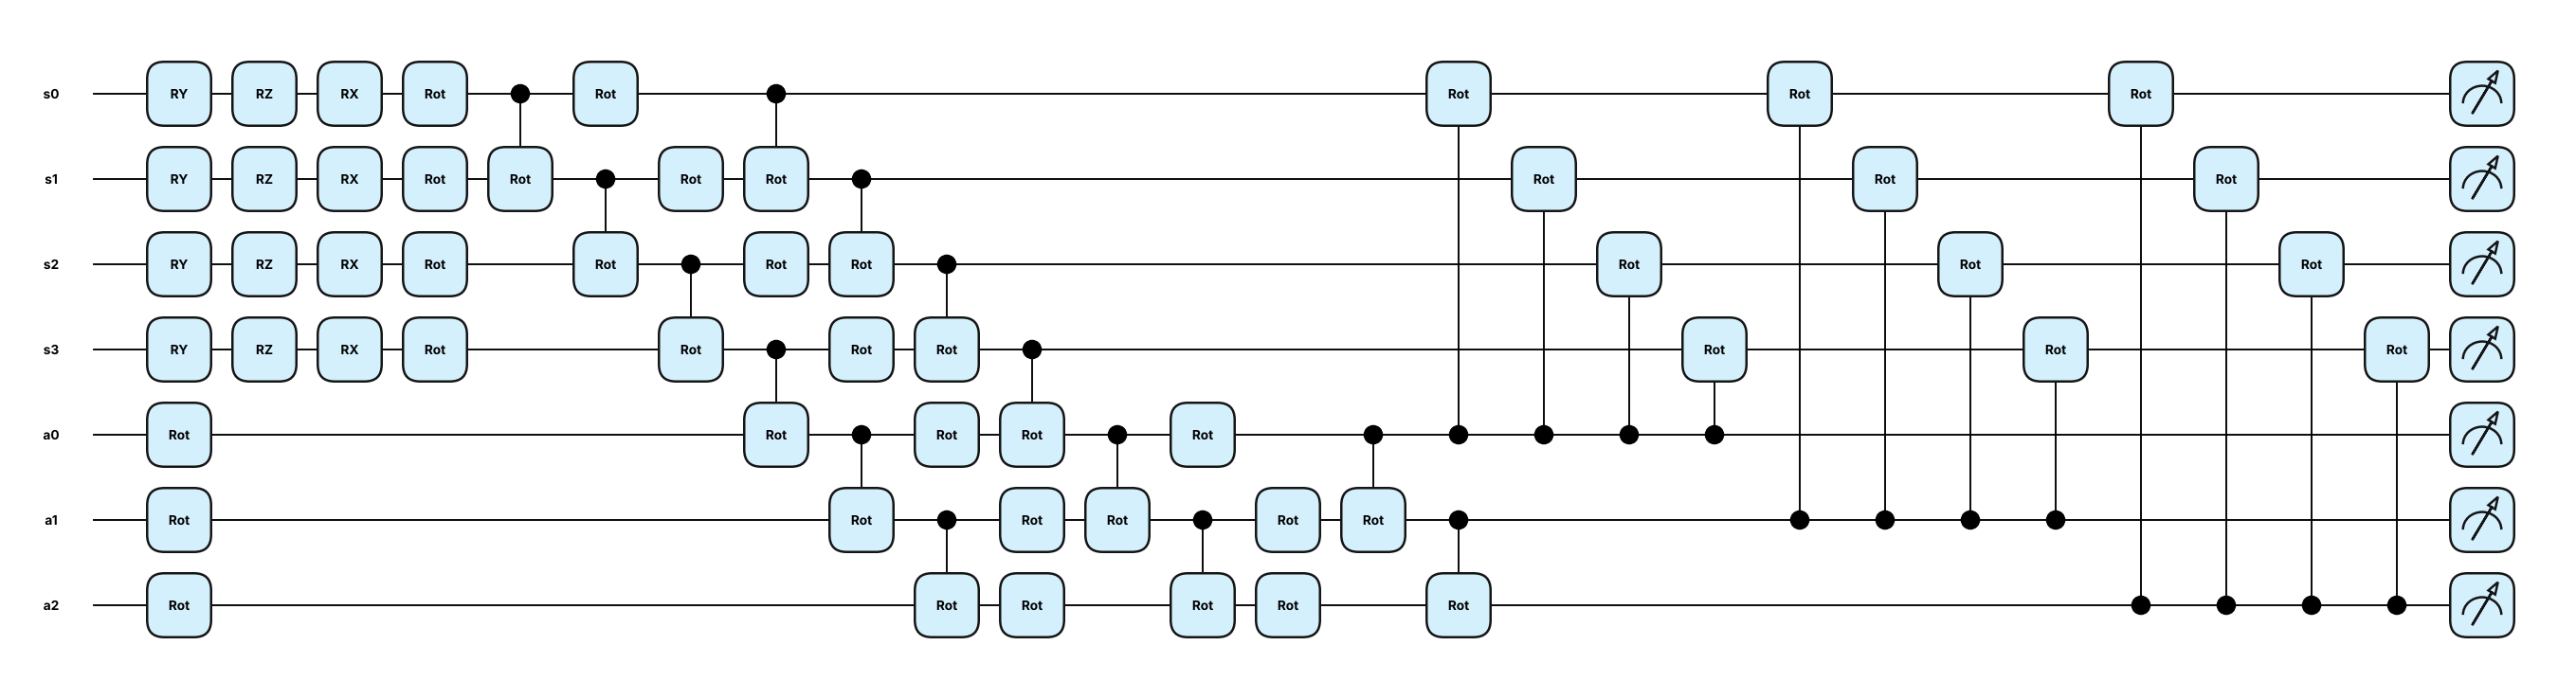
\includegraphics[width=\textwidth]{figures/circuit_one_patch.png}
  \caption{PennyLane drawing of the gates of one patch with $L=2$ repetitions of $W_i$ (the experiments use $L=2$ and $L=4$).}
  \label{fig:onepatch}
\end{figure}

\subsection{MNIST results}

Supplementary Tables~\ref{tab:mnist-results} and~\ref{tab:mnist-amp} give the test accuracies behind Figs.~\ref{fig:capacity} and~\ref{fig:classical}.

\begin{table}[htbp]
  \centering
  \caption{MNIST test accuracy (\%) at the last epoch, mean $\pm$ standard deviation over three seeds. Classical models are sized to the parameter count of the circuit with the given $L$; logistic regression does not depend on $L$. The best mean of each column within each block is in bold. $^\dagger$One of the three seeds stalled at about 47\% training accuracy and is included in the mean. Generated from the result files by \texttt{scripts/paper\_figures.py}.}
  \label{tab:mnist-results}
  \footnotesize
  \setlength{\tabcolsep}{3pt}
  \resizebox{\textwidth}{!}{% generated by scripts/paper_figures.py -- do not edit
\begin{tabular}{@{}lcccccccc@{}}
\toprule
 & \multicolumn{2}{c}{3 vs 5} & \multicolumn{2}{c}{4 vs 9} & \multicolumn{2}{c}{4 classes (0-3)} & \multicolumn{2}{c}{10 classes} \\
\cmidrule(lr){2-3}\cmidrule(lr){4-5}\cmidrule(lr){6-7}\cmidrule(lr){8-9}
 & $8{\times}8$ & $14{\times}14$ & $8{\times}8$ & $14{\times}14$ & $8{\times}8$ & $14{\times}14$ & $8{\times}8$ & $14{\times}14$ \\
\midrule
\multicolumn{9}{@{}l}{\emph{$L=2$ (classical models sized to the circuit with $L=2$)}} \\
serialized, coherent & $96.2\pm0.5$ & $96.9\pm0.2$ & $94.3\pm0.3$ & $96.3\pm0.5$ & $97.4\pm0.2$ & $97.7\pm0.2$ & $89.9\pm0.1$ & $91.8\pm0.2$ \\
serialized, measured & $95.7\pm0.5$ & $96.8\pm0.6$ & $92.6\pm0.4$ & $96.1\pm0.3$ & $90.7\pm4.8$ & $97.0\pm0.1$ & $64.0\pm14.1$$^\dagger$ & $79.9\pm2.8$ \\
MLP, same parameters & $95.6\pm0.1$ & $97.2\pm1.5$ & $95.8\pm0.1$ & $97.3\pm0.6$ & $97.7\pm0.3$ & $98.0\pm0.1$ & $92.0\pm0.2$ & $93.7\pm0.3$ \\
CNN, same parameters & $\mathbf{98.2}\pm0.2$ & $\mathbf{98.5}\pm0.3$ & $\mathbf{96.4}\pm0.2$ & $\mathbf{98.7}\pm0.2$ & $\mathbf{98.7}\pm0.1$ & $\mathbf{99.0}\pm0.1$ & $\mathbf{93.6}\pm0.5$ & $\mathbf{96.3}\pm0.1$ \\
logistic regression & $95.1\pm0.2$ & $95.7\pm0.5$ & $94.8\pm0.2$ & $97.0\pm0.3$ & $97.1\pm0.1$ & $97.5\pm0.1$ & $89.9\pm0.1$ & $91.7\pm0.1$ \\
\midrule
\multicolumn{9}{@{}l}{\emph{$L=4$ (classical models sized to the circuit with $L=4$)}} \\
serialized, coherent & $97.2\pm0.3$ & $97.5\pm0.2$ & $94.9\pm0.3$ & $97.0\pm0.6$ & $97.0\pm0.1$ & $97.8\pm0.3$ & $91.1\pm0.3$ & $92.8\pm0.4$ \\
serialized, measured & $96.9\pm0.2$ & $97.0\pm0.6$ & $94.8\pm0.4$ & $96.8\pm0.3$ & $96.3\pm0.6$ & $97.5\pm0.2$ & $81.2\pm4.1$ & $86.2\pm3.3$ \\
MLP, same parameters & $97.7\pm0.7$ & $98.0\pm0.6$ & $96.8\pm0.3$ & $97.7\pm0.4$ & $98.3\pm0.2$ & $98.3\pm0.0$ & $94.7\pm0.3$ & $95.1\pm0.1$ \\
CNN, same parameters & $\mathbf{98.4}\pm0.4$ & $\mathbf{98.7}\pm0.1$ & $\mathbf{97.0}\pm0.4$ & $\mathbf{98.9}\pm0.2$ & $\mathbf{98.8}\pm0.0$ & $\mathbf{99.1}\pm0.1$ & $\mathbf{95.3}\pm0.2$ & $\mathbf{97.2}\pm0.2$ \\
\bottomrule
\end{tabular}
}
\end{table}

\begin{table}[htbp]
  \centering
  \caption{MNIST test accuracy (\%) of the amplitude-encoding circuits: the whole image as a normalized amplitude vector of 4 qubits (shrunk to $4\times4$) or 7 qubits ($8\times8$ as it is, $14\times14$ shrunk to $11\times11$), followed by $L$ layers of the block of the serialized circuit and the same readout (60--462 parameters). Mean $\pm$ standard deviation over three seeds; the best mean of each column is in bold.}
  \label{tab:mnist-amp}
  \footnotesize
  \setlength{\tabcolsep}{3pt}
  % generated by scripts/paper_figures.py -- do not edit
\begin{tabular}{@{}llcccccccc@{}}
\toprule
 & & \multicolumn{2}{c}{3 vs 5} & \multicolumn{2}{c}{4 vs 9} & \multicolumn{2}{c}{4 classes (0-3)} & \multicolumn{2}{c}{10 classes} \\
\cmidrule(lr){3-4}\cmidrule(lr){5-6}\cmidrule(lr){7-8}\cmidrule(lr){9-10}
qubits & $L$ & $8{\times}8$ & $14{\times}14$ & $8{\times}8$ & $14{\times}14$ & $8{\times}8$ & $14{\times}14$ & $8{\times}8$ & $14{\times}14$ \\
\midrule
4 & 2 & $93.6\pm0.7$ & $93.8\pm0.4$ & $78.0\pm0.6$ & $83.5\pm0.3$ & $88.7\pm0.1$ & $89.2\pm1.1$ & $68.8\pm0.1$ & $72.1\pm1.4$ \\
4 & 4 & $93.9\pm0.2$ & $94.6\pm0.2$ & $79.0\pm1.8$ & $85.0\pm0.4$ & $89.1\pm0.3$ & $90.6\pm0.1$ & $70.5\pm0.7$ & $75.6\pm0.6$ \\
4 & 8 & $94.4\pm0.4$ & $94.6\pm0.2$ & $79.7\pm0.5$ & $85.3\pm1.0$ & $90.0\pm0.4$ & $90.9\pm0.4$ & $72.4\pm0.3$ & $76.4\pm0.9$ \\
\midrule
7 & 2 & $93.5\pm1.4$ & $92.3\pm0.2$ & $88.4\pm0.4$ & $94.9\pm0.4$ & $96.0\pm0.2$ & $96.0\pm0.1$ & $82.4\pm1.2$ & $82.9\pm1.5$ \\
7 & 4 & $94.9\pm1.0$ & $94.6\pm0.8$ & $90.2\pm0.1$ & $\mathbf{95.2}\pm0.1$ & $96.6\pm0.4$ & $96.8\pm0.4$ & $86.3\pm0.2$ & $86.4\pm1.0$ \\
7 & 8 & $\mathbf{96.0}\pm0.5$ & $\mathbf{95.7}\pm0.5$ & $\mathbf{93.5}\pm0.6$ & $\mathbf{95.2}\pm0.5$ & $\mathbf{97.5}\pm0.2$ & $\mathbf{97.1}\pm0.2$ & $\mathbf{87.9}\pm0.4$ & $\mathbf{89.2}\pm0.5$ \\
\bottomrule
\end{tabular}

\end{table}

\subsection{Twelve further datasets}

Supplementary Table~\ref{tab:datasets} describes the datasets and Supplementary Table~\ref{tab:bench} gives the test accuracies behind Fig.~\ref{fig:bench}.

\begin{table}[htbp]
  \centering
  \caption{The twelve further datasets. $d$: features, $N$: patches of four features, $k$: classes. Tabular sets keep their natural class frequencies (majority class in the last column); the image sets are class balanced except PneumoniaMNIST, which keeps its official splits.}
  \label{tab:datasets}
  \footnotesize
  \resizebox{\textwidth}{!}{%
  \begin{tabular}{@{}llrrrrr@{}}
    \toprule
    dataset & source & $d$ & $N$ & $k$ & train / val / test & majority \\
    \midrule
    Waveform & UCI 107~\cite{uci_waveform} (21 wave attributes) & 21 & 6 & 3 & 3\,601 / 400 / 999 & 33.9\% \\
    Wall-Following & UCI 194~\cite{freire2009wall}, 24 sensors & 24 & 6 & 4 & 3\,929 / 436 / 1\,091 & 40.4\% \\
    Covertype & UCI 31~\cite{uci_covertype,blackard1999covertype} & 54 & 14 & 7 & 10\,000 / 2\,000 / 9\,999 & 48.8\% \\
    Letter & UCI 59~\cite{frey1991letter} & 16 & 4 & 26 & 10\,000 / 1\,600 / 4\,000 & 4.1\% \\
    Spambase & UCI 94~\cite{uci_spambase} & 57 & 15 & 2 & 3\,313 / 368 / 920 & 60.5\% \\
    Credit Default & UCI 350~\cite{yeh2009credit} & 23 & 6 & 2 & 10\,000 / 2\,000 / 6\,000 & 77.9\% \\
    Landsat & UCI 146~\cite{uci_landsat,king1995statlog} (train and test joined) & 36 & 9 & 6 & 4\,634 / 514 / 1\,287 & 23.9\% \\
    Dry Bean & UCI 602~\cite{koklu2020drybean} & 16 & 4 & 7 & 9\,801 / 1\,089 / 2\,721 & 26.1\% \\
    \midrule
    Fashion-MNIST & \cite{xiao2017fashion}, $14\times14$ & 196 & 49 & 10 & 10\,000 / 2\,000 / 10\,000 & 10\% \\
    BloodMNIST & MedMNIST v2~\cite{yang2023medmnist,acevedo2020blood}, grayscale, $14\times14$ & 196 & 49 & 8 & 8\,779 / 1\,527 / 3\,421 & 19.5\% \\
    PneumoniaMNIST & MedMNIST v2~\cite{yang2023medmnist,kermany2018pneumonia}, $14\times14$ & 196 & 49 & 2 & 4\,708 / 524 / 624 & 62.5\% \\
    Kuzushiji-MNIST & \cite{clanuwat2018kmnist}, $14\times14$ & 196 & 49 & 10 & 10\,000 / 2\,000 / 10\,000 & 10\% \\
    \bottomrule
  \end{tabular}}
\end{table}

\begin{table}[htbp]
  \centering
  \caption{Test accuracy (\%) on twelve further datasets at the last epoch, mean $\pm$ standard deviation over three seeds; the best mean of each row is in bold. $k$: classes, $N$: patches of four features, params: parameters of the circuit with coherent memory and $L=4$, which is also the size of the MLP and the CNN. Amplitude: the whole input as the amplitude vector of the same seven qubits with $L=4$ or $8$ layers of the same block (200--550 parameters). Gradient boosting: scikit-learn histogram gradient boosting, an ensemble of 300 trees shown as a reference, not tuned. Measured memory was run on the tabular sets only (above the line).}
  \label{tab:bench}
  \footnotesize
  \setlength{\tabcolsep}{2.5pt}
  \resizebox{\textwidth}{!}{% generated by scripts/paper_figures.py -- do not edit
\begin{tabular}{@{}lrrrrrrrrrrr@{}}
\toprule
 & & & & \multicolumn{4}{c}{classical} & \multicolumn{2}{c}{amplitude, 7 qubits} & \multicolumn{2}{c@{}}{serialized, 7 qubits} \\
\cmidrule(lr){5-8}\cmidrule(lr){9-10}\cmidrule(l){11-12}
dataset & $k$ & $N$ & params & logistic & MLP & CNN & grad.\ boost. & $L{=}4$ & $L{=}8$ & \multicolumn{1}{c}{coherent} & \multicolumn{1}{c@{}}{measured} \\
\midrule
Waveform & 3 & 6 & 1056 & $\mathbf{87.2}${\scriptsize$\pm0.1$} & $87.1${\scriptsize$\pm0.8$} & -- & $85.5${\scriptsize$\pm0.5$} & $86.2${\scriptsize$\pm0.2$} & $86.8${\scriptsize$\pm0.6$} & $85.0${\scriptsize$\pm0.2$} & $82.7${\scriptsize$\pm3.1$} \\
Wall-Following & 4 & 6 & 1071 & $68.3${\scriptsize$\pm0.3$} & $91.9${\scriptsize$\pm0.4$} & -- & $\mathbf{99.9}${\scriptsize$\pm0.0$} & $73.0${\scriptsize$\pm1.4$} & $77.1${\scriptsize$\pm1.5$} & $90.1${\scriptsize$\pm0.7$} & $87.0${\scriptsize$\pm2.0$} \\
Covertype & 7 & 14 & 2364 & $71.6${\scriptsize$\pm0.1$} & $75.8${\scriptsize$\pm0.2$} & -- & $\mathbf{82.2}${\scriptsize$\pm0.2$} & $71.7${\scriptsize$\pm0.5$} & $72.0${\scriptsize$\pm0.3$} & $73.8${\scriptsize$\pm0.2$} & $71.7${\scriptsize$\pm0.5$} \\
Letter & 26 & 4 & 1089 & $72.6${\scriptsize$\pm0.2$} & $80.4${\scriptsize$\pm0.8$} & -- & $\mathbf{95.3}${\scriptsize$\pm0.1$} & $59.7${\scriptsize$\pm2.5$} & $63.6${\scriptsize$\pm0.8$} & $71.0${\scriptsize$\pm1.6$} & $63.5${\scriptsize$\pm3.1$} \\
Spambase & 2 & 15 & 2445 & $92.0${\scriptsize$\pm0.1$} & $93.4${\scriptsize$\pm0.5$} & -- & $\mathbf{96.1}${\scriptsize$\pm0.3$} & $90.0${\scriptsize$\pm0.4$} & $90.7${\scriptsize$\pm0.8$} & $91.7${\scriptsize$\pm0.4$} & $93.5${\scriptsize$\pm0.6$} \\
Credit Default & 2 & 6 & 1041 & $81.1${\scriptsize$\pm0.1$} & $81.7${\scriptsize$\pm0.1$} & -- & $81.4${\scriptsize$\pm0.3$} & $79.6${\scriptsize$\pm0.2$} & $79.7${\scriptsize$\pm0.1$} & $81.9${\scriptsize$\pm0.3$} & $\mathbf{82.4}${\scriptsize$\pm0.1$} \\
Landsat & 6 & 9 & 1569 & $82.3${\scriptsize$\pm0.2$} & $89.2${\scriptsize$\pm0.1$} & -- & $\mathbf{92.3}${\scriptsize$\pm0.5$} & $78.7${\scriptsize$\pm0.2$} & $78.9${\scriptsize$\pm0.2$} & $89.3${\scriptsize$\pm1.2$} & $86.8${\scriptsize$\pm1.0$} \\
Dry Bean & 7 & 4 & 804 & $92.1${\scriptsize$\pm0.0$} & $92.3${\scriptsize$\pm0.1$} & -- & $92.8${\scriptsize$\pm0.2$} & $91.8${\scriptsize$\pm0.1$} & $91.8${\scriptsize$\pm0.2$} & $\mathbf{92.9}${\scriptsize$\pm0.2$} & $92.8${\scriptsize$\pm0.0$} \\
\midrule
Fashion-MNIST & 10 & 49 & 7869 & $82.6${\scriptsize$\pm0.2$} & $85.2${\scriptsize$\pm0.1$} & $85.7${\scriptsize$\pm0.6$} & $\mathbf{86.5}${\scriptsize$\pm0.4$} & $73.7${\scriptsize$\pm0.4$} & $74.4${\scriptsize$\pm0.8$} & $82.7${\scriptsize$\pm0.2$} & -- \\
BloodMNIST & 8 & 49 & 7839 & $67.2${\scriptsize$\pm0.4$} & $70.3${\scriptsize$\pm1.2$} & $81.2${\scriptsize$\pm0.4$} & $\mathbf{86.0}${\scriptsize$\pm0.2$} & $58.0${\scriptsize$\pm0.6$} & $60.2${\scriptsize$\pm0.2$} & $73.8${\scriptsize$\pm1.3$} & -- \\
PneumoniaMNIST & 2 & 49 & 7749 & $83.5${\scriptsize$\pm0.1$} & $84.1${\scriptsize$\pm0.9$} & $85.6${\scriptsize$\pm0.8$} & $84.9${\scriptsize$\pm0.0$} & $81.2${\scriptsize$\pm1.5$} & $81.9${\scriptsize$\pm1.2$} & $\mathbf{87.7}${\scriptsize$\pm0.7$} & -- \\
Kuzushiji-MNIST & 10 & 49 & 7869 & $68.2${\scriptsize$\pm0.3$} & $78.7${\scriptsize$\pm0.2$} & $80.3${\scriptsize$\pm1.5$} & $\mathbf{83.4}${\scriptsize$\pm0.3$} & $58.3${\scriptsize$\pm0.8$} & $62.6${\scriptsize$\pm0.8$} & $70.4${\scriptsize$\pm0.7$} & -- \\
\bottomrule
\end{tabular}
}
\end{table}

\begin{table}[htbp]
  \centering
  \caption{As Supplementary Table~\ref{tab:bench}, but balanced accuracy (\%), the mean of the per-class recalls: last epoch, mean $\pm$ standard deviation over three seeds; the best mean of each row is in bold.}
  \label{tab:bench-bal}
  \footnotesize
  \setlength{\tabcolsep}{2.5pt}
  \resizebox{\textwidth}{!}{% generated by scripts/paper_figures.py -- do not edit
\begin{tabular}{@{}lrrrrrrrrrrr@{}}
\toprule
 & & & & \multicolumn{4}{c}{classical} & \multicolumn{2}{c}{amplitude, 7 qubits} & \multicolumn{2}{c@{}}{serialized, 7 qubits} \\
\cmidrule(lr){5-8}\cmidrule(lr){9-10}\cmidrule(l){11-12}
dataset & $k$ & $N$ & params & logistic & MLP & CNN & grad.\ boost. & $L{=}4$ & $L{=}8$ & \multicolumn{1}{c}{coherent} & \multicolumn{1}{c@{}}{measured} \\
\midrule
Waveform & 3 & 6 & 1056 & $\mathbf{87.2}${\scriptsize$\pm0.1$} & $87.1${\scriptsize$\pm0.8$} & -- & $85.5${\scriptsize$\pm0.5$} & $86.2${\scriptsize$\pm0.2$} & $86.8${\scriptsize$\pm0.6$} & $85.0${\scriptsize$\pm0.2$} & $82.7${\scriptsize$\pm3.1$} \\
Wall-Following & 4 & 6 & 1071 & $59.7${\scriptsize$\pm1.0$} & $90.8${\scriptsize$\pm0.9$} & -- & $\mathbf{99.9}${\scriptsize$\pm0.0$} & $66.2${\scriptsize$\pm1.8$} & $69.9${\scriptsize$\pm0.9$} & $88.8${\scriptsize$\pm0.8$} & $84.6${\scriptsize$\pm2.7$} \\
Covertype & 7 & 14 & 2364 & $46.0${\scriptsize$\pm1.2$} & $56.2${\scriptsize$\pm2.4$} & -- & $\mathbf{67.8}${\scriptsize$\pm0.2$} & $42.3${\scriptsize$\pm0.1$} & $42.1${\scriptsize$\pm1.7$} & $45.3${\scriptsize$\pm1.2$} & $38.1${\scriptsize$\pm2.6$} \\
Letter & 26 & 4 & 1089 & $72.5${\scriptsize$\pm0.2$} & $80.4${\scriptsize$\pm0.8$} & -- & $\mathbf{95.3}${\scriptsize$\pm0.1$} & $59.6${\scriptsize$\pm2.4$} & $63.5${\scriptsize$\pm0.7$} & $70.8${\scriptsize$\pm1.6$} & $63.5${\scriptsize$\pm3.1$} \\
Spambase & 2 & 15 & 2445 & $91.2${\scriptsize$\pm0.1$} & $92.9${\scriptsize$\pm0.4$} & -- & $\mathbf{96.1}${\scriptsize$\pm0.3$} & $89.2${\scriptsize$\pm0.5$} & $90.0${\scriptsize$\pm0.8$} & $91.4${\scriptsize$\pm0.8$} & $93.1${\scriptsize$\pm0.7$} \\
Credit Default & 2 & 6 & 1041 & $61.2${\scriptsize$\pm0.2$} & $65.4${\scriptsize$\pm0.3$} & -- & $65.0${\scriptsize$\pm0.2$} & $58.5${\scriptsize$\pm0.4$} & $59.1${\scriptsize$\pm0.3$} & $65.3${\scriptsize$\pm0.7$} & $\mathbf{66.3}${\scriptsize$\pm0.4$} \\
Landsat & 6 & 9 & 1569 & $74.7${\scriptsize$\pm0.4$} & $86.5${\scriptsize$\pm0.1$} & -- & $\mathbf{90.1}${\scriptsize$\pm0.6$} & $69.3${\scriptsize$\pm0.2$} & $69.4${\scriptsize$\pm0.2$} & $86.8${\scriptsize$\pm1.4$} & $83.6${\scriptsize$\pm1.3$} \\
Dry Bean & 7 & 4 & 804 & $93.4${\scriptsize$\pm0.0$} & $93.5${\scriptsize$\pm0.0$} & -- & $93.8${\scriptsize$\pm0.2$} & $92.9${\scriptsize$\pm0.2$} & $93.0${\scriptsize$\pm0.1$} & $\mathbf{93.9}${\scriptsize$\pm0.2$} & $93.8${\scriptsize$\pm0.1$} \\
\midrule
Fashion-MNIST & 10 & 49 & 7869 & $82.6${\scriptsize$\pm0.2$} & $85.2${\scriptsize$\pm0.1$} & $85.7${\scriptsize$\pm0.6$} & $\mathbf{86.5}${\scriptsize$\pm0.4$} & $73.7${\scriptsize$\pm0.4$} & $74.4${\scriptsize$\pm0.8$} & $82.7${\scriptsize$\pm0.2$} & -- \\
BloodMNIST & 8 & 49 & 7839 & $67.2${\scriptsize$\pm0.4$} & $69.8${\scriptsize$\pm1.1$} & $79.5${\scriptsize$\pm0.4$} & $\mathbf{84.8}${\scriptsize$\pm0.3$} & $55.5${\scriptsize$\pm0.5$} & $57.4${\scriptsize$\pm1.1$} & $73.0${\scriptsize$\pm1.1$} & -- \\
PneumoniaMNIST & 2 & 49 & 7749 & $78.9${\scriptsize$\pm0.2$} & $79.3${\scriptsize$\pm1.4$} & $81.2${\scriptsize$\pm1.2$} & $80.8${\scriptsize$\pm0.0$} & $76.1${\scriptsize$\pm2.1$} & $77.0${\scriptsize$\pm1.8$} & $\mathbf{84.0}${\scriptsize$\pm1.0$} & -- \\
Kuzushiji-MNIST & 10 & 49 & 7869 & $68.2${\scriptsize$\pm0.3$} & $78.7${\scriptsize$\pm0.2$} & $80.3${\scriptsize$\pm1.5$} & $\mathbf{83.4}${\scriptsize$\pm0.3$} & $58.3${\scriptsize$\pm0.8$} & $62.6${\scriptsize$\pm0.8$} & $70.4${\scriptsize$\pm0.7$} & -- \\
\bottomrule
\end{tabular}
}
\end{table}

\subsection{Classical models with the structure of the circuit}

\begin{table}[htbp]
  \centering
  \caption{The serialized circuit ($L=4$) against classical models that read the input patch by patch with position-specific parameters. Test accuracy (\%) at the last epoch, mean over three seeds; the best mean of each row is in bold. MLP: the one-hidden-layer MLP of Supplementary Table~\ref{tab:bench} (for MNIST, the parameter-matched MLP of Supplementary Table~\ref{tab:mnist-results}). Seq.\ RNN: recurrent network with its own weights at every patch; MPS: matrix-product-state classifier with one tensor per feature; both are sized to the parameter count of the circuit as closely as their hidden or bond dimension allows. 8-state HMM: input-driven hidden Markov model over eight states, with 1.5 to 2 times the parameters of the circuit. The learning rate of each classical model is chosen by mean validation accuracy. Measured memory was not run on the 49-patch image sets.}
  \label{tab:struct}
  \footnotesize
  % generated by scripts/paper_figures.py -- do not edit
\begin{tabular}{@{}lrrrrrr@{}}
\toprule
 & \multicolumn{2}{c}{serialized circuit} & \multicolumn{4}{c@{}}{classical} \\
\cmidrule(lr){2-3}\cmidrule(l){4-7}
dataset & coherent & measured & MLP & seq.\ RNN & MPS & 8-state HMM \\
\midrule
Waveform & $85.0$ & $82.7$ & $87.1$ & $87.4$ & $\mathbf{87.5}$ & $84.9$ \\
Wall-Following & $90.1$ & $87.0$ & $91.9$ & $93.1$ & $\mathbf{95.2}$ & $85.7$ \\
Covertype & $73.8$ & $71.7$ & $\mathbf{75.8}$ & $75.3$ & $75.2$ & $71.3$ \\
Letter & $71.0$ & $63.5$ & $80.4$ & $\mathbf{80.7}$ & $71.4$ & $53.8$ \\
Spambase & $91.7$ & $93.5$ & $93.4$ & $93.2$ & $\mathbf{93.8}$ & $92.5$ \\
Credit Default & $81.9$ & $\mathbf{82.4}$ & $81.7$ & $82.2$ & $82.0$ & $81.9$ \\
Landsat & $89.3$ & $86.8$ & $89.2$ & $\mathbf{89.7}$ & $89.6$ & $83.7$ \\
Dry Bean & $\mathbf{92.9}$ & $92.8$ & $92.3$ & $92.8$ & $\mathbf{92.9}$ & $91.9$ \\
Fashion-MNIST & $82.7$ & -- & $\mathbf{85.2}$ & $77.1$ & $82.2$ & $53.0$ \\
BloodMNIST & $\mathbf{73.8}$ & -- & $70.3$ & $64.7$ & $71.9$ & $44.9$ \\
PneumoniaMNIST & $\mathbf{87.7}$ & -- & $84.1$ & $87.6$ & $87.5$ & $82.9$ \\
Kuzushiji-MNIST & $70.4$ & -- & $\mathbf{78.7}$ & $61.8$ & $62.1$ & $31.0$ \\
MNIST $8\times8$, 3 vs.\ 5 & $97.2$ & $96.9$ & $97.7$ & $\mathbf{98.1}$ & $97.4$ & $65.0$ \\
MNIST $8\times8$, 10 classes & $91.1$ & $81.2$ & $\mathbf{94.7}$ & $92.7$ & $92.1$ & $68.2$ \\
\bottomrule
\end{tabular}

\end{table}

\subsection{Readout and head variants on Letter}

Supplementary Table~\ref{tab:letter} collects the variants of the circuit run on Letter, each against a one-hidden-layer MLP with the same number of parameters.

\begin{table}[htbp]
  \centering
  \caption{Letter (26 classes): readout, head and depth variants of the circuit with coherent memory, against a one-hidden-layer MLP of the same size. Test accuracy (\%), mean $\pm$ standard deviation over three seeds; the better mean of each row is in bold. Gradient-boosted trees reach $95.3\pm0.1$.}
  \label{tab:letter}
  \footnotesize
  % generated by scripts/paper_figures.py -- do not edit
\begin{tabular}{@{}lrlrl@{}}
\toprule
 & \multicolumn{2}{c}{circuit} & \multicolumn{2}{c@{}}{MLP, same size} \\
\cmidrule(lr){2-3}\cmidrule(l){4-5}
readout and head & params & accuracy & params & accuracy \\
\midrule
$Z$, $ZZ$ (14 features), linear head, $L=4$ & 1\,089 & $71.0\pm1.6$ & 1\,101 & $\mathbf{80.4}\pm0.8$ \\
$Z$, $ZZ$ (14 features), linear head, $L=9$ & 1\,869 & $71.8\pm2.1$ & -- & -- \\
$+X$, $XX$, $Y$, $YY$ (42 features), linear head, $L=4$ & 1\,817 & $79.9\pm0.2$ & 1\,832 & $\mathbf{84.7}\pm1.2$ \\
$Z$, $ZZ$ (14 features), MLP head (64 units), $L=4$ & 3\,349 & $85.6\pm0.6$ & 3\,337 & $\mathbf{87.8}\pm0.2$ \\
\bottomrule
\end{tabular}

\end{table}

\subsection{$28\times28$ images}
\label{sec:supp-28}

At $28\times28$ the serialized circuit has 196 patches and 74\% of them are empty (62\% at $14\times14$, 41\% at $8\times8$). With the settings of the MNIST experiments it stays at chance or only fits the training set, and the simulation takes about 47 minutes (3 vs.\ 5) to 2 hours (10 classes) per epoch, i.e.\ days per run, so it is not reported. The classical and amplitude-encoding baselines were run at $28\times28$ and are in the code repository.


\end{document}
